%theory

\part{Theoretical Background}
\label{sec:theory}

\acresetall

\chapter{Graph Theory}
\label{sec:graphtheory}

Graph theory is used intensively in this thesis, therefore a small introduction
to this field is provided. Graph theory is a powerful mathematical tool to
describe relations between pairs of objects. Its biggest advantage is the broad
range of applicability in fields like computer science, biology, social sciences
and of course physics and chemistry. In the following sections the focus will be
put on introducing graph theory in general and demonstrating its usefulness in
the scope of this thesis. If not mentioned otherwise the chapter is mainly based
on standard books on graph theory by
\citeauthor{West_Introductiongraphtheory_2001}\autocite{West_Introductiongraphtheory_2001}
and
\citeauthor{Balakrishnan_Schaumoutlinetheory_1997}\autocite{Balakrishnan_Schaumoutlinetheory_1997}.

\section{The Definition of a Graph}
\label{sec:DefinitionGraph}

The foundations for graph theory were laid out by Euler in his famous solution
to the K\"onigsberg Bridge Problem\autocite{Euler_Solutioproblematisad_1741}.
The problem at hand was concerned with a specific bridge layout that connected
the island Kneiphopf with the rest of the mainlands of the city of K\"onigsberg
via seven bridges.
%
\begin{figure}[htb]
    \centering
    \subfloat[\label{subfig:koenigsberg-scheme}]{
        \begin{tikzpicture}
            \node[anchor=south west, inner sep=0] at (0,0) {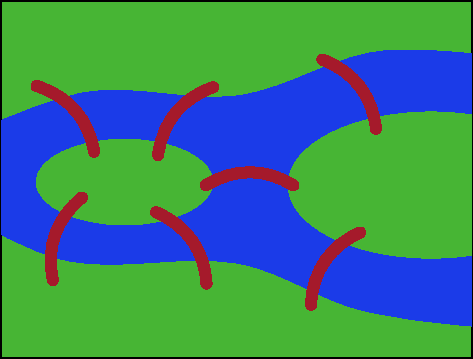
\includegraphics[width=.39\textwidth]{other-pics/koenigsberg-scheme.pdf}};
            \node at (1.2,1.8) {A};
            \node at (4,1.8) {B};
            \node at (1.7,3) {C};
            \node at (1.7,0.5) {D};
        \end{tikzpicture}
    }\hspace{0.05\textwidth}
    \subfloat[\label{subfig:koenigsberg-graph}]{
        \begin{tikzpicture}
            \node[main node,scale=0.75] (A) {A};
            \node[main node,scale=0.75] (B) [right = 2cm of A] {B};
            \node[right = 1cm of A] (dummy)  {};
            \node[main node,scale=0.75] (C) [above = 1cm of dummy] {C};
            \node[main node,scale=0.75] (D) [below = 1cm of dummy] {D};

            \path[draw,thick]
            (A) edge node {} (B)            
            (C) edge node {} (B)            
            (D) edge node {} (B)            
            (A) edge[bend right] node {} (C)            
            (A) edge[bend right=60] node {} (D)            
            (A) edge[bend left=60] node {} (C)            
            (A) edge[bend left] node {} (D)            
            ;

        \end{tikzpicture}
    }
    \caption{The K\"onigsberg Bridge Problem.
    \protect\subref{subfig:koenigsberg-scheme} Schematic representation of the
    bridge layout of K\"onigsberg with the river Pregel (blue), landmasses
    (green) and bridges (red), and \protect\subref{subfig:koenigsberg-graph}
    respective graph drawing.}
    \label{fig:KoenigsbergBridgeProblem}
\end{figure}
%
The bridge layout is depicted schematically in
figure~\ref{subfig:koenigsberg-scheme}. Is it possible for a citizen of
K\"onigsberg to leave home, cross each bridge exactly once and return? The
answer is no and it was proven by Euler using a reduction of the problem as
shown in figure~\ref{subfig:koenigsberg-graph}. Landmasses are reduced to
circles and their connections via bridges is shown as lines between them. This
simplification makes it easy to realise why the answer to the formerly posed
question is no. It is clear that each the landmasses would need to be connected
by an even number of bridges for the desired traversal to exist.

Mathematically, a \textit{graph} $G$ is a triple that contains a \textit{vertex
set} $N(G)$, an \textit{edge set} $E(G)$, and a relation that associates two
vertices (not necessarily distinct) with each edge, i.e. that connects pairs of
vertices via their endpoints. Edges can form a \textit{loop} by having both
endpoints at the same vertex and multiple edges can connect the same vertices.
However, \textit{simple graphs} do not contain loops and multiple edges and are
more important for most practical applications. A simple graph can now be
defined by a set of unordered pairs of vertices by defining each edge as $e=uv$
or $e=vu$ with $u$ and $v$ being the endpoints (or vertices) of the edges. Then,
neighbouring or adjacent vertices are those that share an edge.

Graphs are often just represented as a graph drawing such as
figure~\ref{subfig:koenigsberg-graph}, however, sometimes it can be useful to
introduce a matrix representation. A simple graph $G$ with vertex set
$N(G)=\{v_1,v_2,\dots,v_n\}$ and edge set $E(G)=\{e_1,e_2,\dots,e_m\}$ can be
defined by writing an \textit{adjacency matrix} $\mathbf{A}$ that encodes the
edge-connectivity of the vertex set, i.e. $\mathbf{A}$ is a $n\times n$ matrix
where each matrix element $A_{ij}$ represents the number of edges that connect
$v_i$ and $v_j$. For the K\"onigsberg Bridge problem one possible adjacency
matrix that corresponds to ordering the vertices alphabetically by their label
is:
%
\begin{equation}
    \mathbf{A}=
    \begin{pmatrix}
         0 & 1 & 2 & 2\\
         1 & 0 & 1 & 1\\
         2 & 1 & 0 & 0\\
         2 & 1 & 0 & 0
    \end{pmatrix}.
\end{equation}
%
An adjacency matrix is always symmetric and it can be used to easily determine
the \textit{vertex degree}, that is the number of edges connected to a
particular vertex, by calculating the sum over all entries in the corresponding
row or column. 

Alternatively, the \textit{incidence matrix} $M$ is an $n \cross m$ matrix where
each matrix element $m_{ij}$ is either $1$ or $0$ depending on whether $v_i$ is
an endpoint of $e_j$. If the matrix element $m_{ij}$ is $1$ the vertex $v_i$ and
edge $e_j$ are incident.

The labelling of the vertices in figure~\ref{subfig:koenigsberg-graph} is
arbitrary and so is the ordering of the rows and columns in the adjacency
matrix. It is clear that a different ordering still describes the same graph
object and should therefore have no influence on the properties of the graph.
Permutation of the vertex labelling for a given simple graph $G$ that turns the
vertex set $N(G)$ into the vertex set $N(H)$ is called a \textit{bijection}. If
such a bijection exists the graphs $G$ and $H$ are \emph{isomorphic} to each
other. This property is important for the discussion of a specific type of
cluster later on in this thesis (chapter~\ref{sec:SHSClusters}).

If it is possible to order the vertices of a simple graph in such a way that
only two consecutively listed vertices are adjacent, the graph can be called a
\textit{path}. An extension of this concept is the \textit{cycle}, that requires
an equal number of vertices and edges so that the graph can be drawn as a circle
of sequentially listed vertices. Consequently, removing an edge from a cycle
always yields a path. In many applications (e.g. road networks) it is not
necessary for the whole graph to represent a path or a cycle, but it is only
important whether the graph contains a path or a cycle. If the graph $G$
contains the graph $H$, $H$ is called a sub-graph of $G$. This requires the
vertex set of $H$ to be contained in $N(G)$ ($N(H)\subseteq N(G)$) as well as
the edge set $E(H)$ ($E(H)\subseteq E(G)$) as well as the assignment of the
endpoints to be the same.

The K\"onigsberg Bridge Problem is not only concerned with the nature of the
bridging network, but more so with how to traverse over it. In graph theoretical
terms the desired solution is called a closed trail, which is a special case of
a walk, where no edge can be repeated (i.e. no bridge can be crossed twice) and
the endpoints have to be the same
vertex.{\interfootnotelinepenalty=10000\footnote{A graph that contains such a
closed tail traversing all edges is also called Eulerian in honour of of Euler's
significant contribution to solve this long-standing problem.}} A walk describes
a way to traverse over a graph by defining a list of vertices and edges
$v_0,e_1,v_1,\dots,e_k,v_k$ where the endpoints for each edge $e_i$ have to be
$v_{i-1}$ and $v_i$ ($1\leq i\leq k$). One possible trail (excluding one bridge)
is shown in figure~\ref{subfig:adtrail}. 
%
\begin{figure}[htb]
    \centering
    \subfloat[A,D-trail\label{subfig:adtrail}]{
        \begin{tikzpicture}
            \node[main node,scale=0.75] (A) {A};
            \node[main node,scale=0.75] (B) [right = 2cm of A] {B};
            \node[right = 1cm of A] (dummy)  {};
            \node[main node,scale=0.75] (C) [above = 1cm of dummy] {C};
            \node[main node,scale=0.75] (D) [below = 1cm of dummy] {D};
        
            \draw[blue,directed,thick] (A) -- (B);
            \draw[blue,directed,thick] (A) to [out=100,in=170] (C);    
            \draw[blue,directed,thick] (C) to [out=260,in=10] (A);    
            \draw[blue,directed,thick] (D) to [out=100,in=350] (A);    
            \draw[blue,directed,thick] (A) to [out=260,in=190] (D);    
            \draw[blue,directed,thick] (B) -- (D);    
            \draw[red,crossed,thick] (B) -- (C);    
        \end{tikzpicture}
    }\hspace{0.5cm}
    \subfloat[C,A-walk\label{subfig:cawalk}]{
        \begin{tikzpicture}
            \node[main node,scale=0.75] (A) {A};
            \node[main node,scale=0.75] (B) [right = 2cm of A] {B};
            \node[right = 1cm of A] (dummy)  {};
            \node[main node,scale=0.75] (C) [above = 1cm of dummy] {C};
            \node[main node,scale=0.75] (D) [below = 1cm of dummy] {D};

            \draw[blue,directed,thick] (C) to [in=100,out=170] (A);
            \draw[blue,directed,thick] (A) to [out=260,in=190] (D);    
            \draw[blue,bidirected,thick] (D) -- (B);    
            \draw[blue,directed,thick] (B) -- (C);    
            \draw[blue,directed,thick] (C) to [out=260,in=10] (A);    
            \draw[blue,directed,thick] (D) to [out=100,in=350] (A);    
            \draw[blue,directed,thick] (A) -- (B);
        \end{tikzpicture}
    }\hspace{0.5cm}
    \subfloat[A,C-path\label{subfig:acpath}]{
        \begin{tikzpicture}
            \node[main node,scale=0.75] (A) {A};
            \node[main node,scale=0.75] (B) [right = 2cm of A] {B};
            \node[right = 1cm of A] (dummy)  {};
            \node[main node,scale=0.75] (C) [above = 1cm of dummy] {C};
            \node[main node,scale=0.75] (D) [below = 1cm of dummy] {D};

            \draw[red,crossed,thick] (A) -- (B);
            \draw[red,crossed,thick] (A) to [out=100,in=170] (C);    
            \draw[red,crossed,thick] (C) to [out=260,in=10] (A);    
            \draw[red,crossed,thick] (D) to [out=100,in=350] (A);    
            \draw[blue,directed,thick] (A) to [out=260,in=190] (D);    
            \draw[blue,directed,thick] (D) -- (B);    
            \draw[blue,directed,thick] (B) -- (C);    
        \end{tikzpicture}
    }
    \caption{Example of one possible \protect\subref{subfig:adtrail} trail,
    \protect\subref{subfig:cawalk} walk and \protect\subref{subfig:acpath} path
    over the bridges of K\"onigsberg. Traversal is in direction of the arrows.
    Red edges indicate not-traversed bridges.}
    \label{fig:walkkoenigsberg}
\end{figure}
%
For simple graphs walks and trails can be specified by listing only vertices,
as there can only be one incoming and one outgoing edge per vertex and no
loops. A short hand notation for such a trail or walk can be given by stating
its endpoints, e.g. A,D-trail, however there is usually more than one way this
trail could be laid out. While trails don't allow for repeated traversal of one
edge, paths require all vertex traversals to be distinct. 

The definition of a path can also be used to define whether a graph is
\emph{connected}. In simple terms a graph is connected if there is a path
leading from each vertex to each other one, hence, for all $u,v\in N(G)$ there
must be a $u,v$-path for $G$ to be connected. An example of a disconnected graph
is shown in figure~\ref{fig:disconnectedgraph}.
%
\begin{figure}[htb]
    \centering
    \begin{tikzpicture}
        \node[main node,scale=0.75] (A) {A};
        \node[main node,scale=0.75] (B) [right = 2cm of A] {B};
        \node[right = 1cm of A] (dummy)  {};
        \node[main node,scale=0.75] (C) [above = 1cm of dummy] {C};
        \node[main node,scale=0.75] (D) [below = 1cm of dummy] {D};
        \node (Comp1) [transform shape=false, draw, color=black, dashed, thick,%
            fit= (A) (C) (D)] {};
        \node (Comp1) [transform shape=false, draw, color=black, dashed, thick,%
            fit= (B)] {};

        \path[draw,thick] (A) edge[bend right] node {} (C) (A) edge[bend right=60] node {} (D) (A) edge[bend left=60] node {} (C)(A) edge[bend left] node {} (D);
    \end{tikzpicture} 
    \caption{Example of a disconnected graph with two components. The vertex B
    has no path to any of the other vertices, therefore the graph is
    disconnected. Adding one edge from B to any other vertex would make this
    graph connected. As a result from being disconnected the graph consists of
    two components (dashed lines; one contains only the vertex B and the other
    one contains the other three vertices.} \label{fig:disconnectedgraph}
\end{figure}
%
The maximally connected sub-graphs of a graph are called its
\textit{components}. In figure~\ref{fig:disconnectedgraph} the vertex B forms
one component, while the rest of the vertices form a second one. The vertex B is
an \textit{isolated vertex} as it is of degree zero. A graph consisting of only
isolated vertices is called a \textit{trivial graph} with each vertex forming
its own trivial component.

Adding edges to any graph either reduces the number of components by 1 or 0,
and therefore the minimum number of components is at least $n-m$. This can be
seen by considering a trivial graph of $n$ vertices and adding $m$ edges such
that the number of components $k$ changes by one with each of the $m$ edges. An
edge that increases the number of components upon deletion is also called a
\textit{cut-edge}.

An important concept utilised in chapter~\ref{sec:thegregorynewtonclusters} of
this thesis is that of induced sub-graphs. If a list of vertices $T$ is removed
from a graph $G$ the vertex-induced sub-graph $H$ with the vertex set
$N(H)=N(G)-T$ is obtained. All edges incident to the removed vertices need to be
removed as well. Removing the edge set $S$ results in the edge-induced sub-graph
$I$ with the edge set $E(I)=E(G)-S$, which leaves the vertex set unchanged.

\section{Planar Graphs}
\label{sec:PlanarGraphs}

\textit{Planar graphs} are of particular importance in chemistry and physics,
especially when studying clusters and complexes that are related to polyhedral
arrangements.  A planar graph $G$ is defined as a graph that can be drawn such
that none of its edges intercept (except at vertices to which both edges are
incident). If a planar graph is drawn in that way it's called a \textit{plane
graph}, while any way of drawing that graph in the 2D plane may be referred to
as a \textit{planar embedding}.

The importance of planar graphs in cluster sciences stems from the fact that
they are related to convex polyhedra. According to \emph{Steinitz's fundamental
theorem on convex types} a graph $G$ is isomorphic to a graph $G(P)$ of a convex
polyhedron $P$ if $G$ is planar and 3-connected. A connected graph $G$ is said
to be $k$-vertex-connected (or $k$-connected) if it has more than $k$ vertices
and remains connected whenever fewer than $k$ vertices are removed. A famous
special case is a cubic graph with every vertex having degree three. Steinitz's
theorem can be illustrated by the following procedure. Take a convex polyhedron
like the icosahedron and remove one face (figure~\ref{subfig:icopoly}). 
%
\begin{figure}[htb]
    \centering
    \tdplotsetmaincoords{60}{0}
    \def \ico {1.618}
    \subfloat[\label{subfig:icopoly}]{
    \begin{tikzpicture}[tdplot_main_coords,
        every node/.style = {circle, fill = blue!20, inner sep = 0pt, minimum size = 0.5cm},
        rotate = 0,
        line join=bevel]

        %\draw[red,->] (0,0,0) -- (0,0,1) node {$z$};
        %\draw[red,->] (0,0,0) -- (0,1,0) node {$y$};
        %\draw[red,->] (0,0,0) -- (1,0,0) node {$x$};

        \coordinate (1) at (0, 1, \ico);
        \coordinate (2) at (0, 1, -\ico);
        \coordinate (3) at (0, -1, \ico);
        \coordinate (4) at (0, -1, -\ico);
        \coordinate (5) at (1, \ico, 0);
        \coordinate (6) at (1, -\ico, 0);
        \coordinate (7) at (-1, \ico, 0);
        \coordinate (8) at (-1, -\ico, 0);
        \coordinate (9) at (\ico, 0, 1);
        \coordinate (10) at (\ico, 0, -1);
        \coordinate (11) at (-\ico, 0, 1);
        \coordinate (12) at (-\ico, 0, -1);

        
        %\foreach \n in {1,...,12}
        %    \node at (\n) {\n};

        \draw[thick, fill=blue!50, opacity=0.75] (3) -- (6) -- (8) -- cycle;
        \draw[thick, fill=blue!50, opacity=0.75] (3) -- (6) -- (9) -- cycle;
        \draw[thick, fill=blue!50, opacity=0.75] (6) -- (10) -- (9) -- cycle;
        \draw[thick, fill=blue!50, opacity=0.75] (1) -- (9) -- (3) -- cycle;
        \draw[thick, fill=blue!50, opacity=0.75] (3) -- (8) -- (11) -- cycle;
        \draw[thick, fill=blue!50, opacity=0.75] (1) -- (11) -- (3) -- cycle;
        \draw[thick, fill=blue!50, opacity=0.75] (1) -- (11) -- (7) -- cycle;
        \draw[thick, fill=blue!50, opacity=0.75] (8) -- (6) -- (4) -- cycle;
        \draw[thick, fill=blue!50, opacity=0.75] (10) -- (6) -- (4) -- cycle;
        \draw[thick, fill=blue!50, opacity=0.75] (12) -- (8) -- (4) -- cycle;
        \draw[thick, fill=blue!50, opacity=0.75] (12) -- (8) -- (11) -- cycle;
        \draw[thick, fill=blue!50, opacity=0.75] (12) -- (7) -- (11) -- cycle;
        \draw[thick, fill=blue!50, opacity=0.75] (12) -- (7) -- (2) -- cycle;
        \draw[thick, fill=blue!50, opacity=0.75] (12) -- (2) -- (4) -- cycle;
        \draw[thick, fill=blue!50, opacity=0.75] (10) -- (2) -- (4) -- cycle;
        \draw[thick, fill=white, opacity=0.5] (5) -- (7) -- (2) -- cycle;
        \draw[thick, fill=blue!50, opacity=0.75] (5) -- (10) -- (9) -- cycle;
        \draw[thick, fill=blue!50, opacity=0.75] (1) -- (7) -- (5) -- cycle;
        \draw[thick, fill=blue!50, opacity=0.75] (5) -- (10) -- (2) -- cycle;
        \draw[thick, fill=blue!50, opacity=0.75] (1) -- (9) -- (5) -- cycle;
    \end{tikzpicture}
    }
    \subfloat[\label{subfig:icostretch1}]{
    \begin{tikzpicture}[tdplot_main_coords,
        every node/.style = {circle, fill = blue!20, inner sep = 0pt, minimum size = 0.5cm},
        rotate = 0,
        line join=bevel]

        %\draw[red,->] (0,0,0) -- (0,0,1) node {$z$};
        %\draw[red,->] (0,0,0) -- (0,1,0) node {$y$};
        %\draw[red,->] (0,0,0) -- (1,0,0) node {$x$};

        \coordinate (1) at (0, 1, \ico);
        \coordinate (2) at (0, -0.4142, -\ico);
        \coordinate (3) at (0, -1, \ico);
        \coordinate (4) at (0, -1, -\ico);
        \coordinate (5) at (2, 2.618, 0);
        \coordinate (6) at (1, -\ico, 0);
        \coordinate (7) at (-2, 2.618, 0);
        \coordinate (8) at (-1, -\ico, 0);
        \coordinate (9) at (\ico, 0, 1);
        \coordinate (10) at (\ico, 0, -1);
        \coordinate (11) at (-\ico, 0, 1);
        \coordinate (12) at (-\ico, 0, -1);

        
        %\foreach \n in {1,...,12}
        %    \node at (\n) {\n};

        \draw[thick, fill=blue!50, opacity=0.75] (3) -- (6) -- (8) -- cycle;
        \draw[thick, fill=blue!50, opacity=0.75] (3) -- (6) -- (9) -- cycle;
        \draw[thick, fill=blue!50, opacity=0.75] (6) -- (10) -- (9) -- cycle;
        \draw[thick, fill=blue!50, opacity=0.75] (1) -- (9) -- (3) -- cycle;
        \draw[thick, fill=blue!50, opacity=0.75] (3) -- (8) -- (11) -- cycle;
        \draw[thick, fill=blue!50, opacity=0.75] (1) -- (11) -- (3) -- cycle;
        \draw[thick, fill=blue!50, opacity=0.75] (1) -- (11) -- (7) -- cycle;
        \draw[thick, fill=blue!50, opacity=0.75] (8) -- (6) -- (4) -- cycle;
        \draw[thick, fill=blue!50, opacity=0.75] (10) -- (6) -- (4) -- cycle;
        \draw[thick, fill=blue!50, opacity=0.75] (12) -- (8) -- (4) -- cycle;
        \draw[thick, fill=blue!50, opacity=0.75] (12) -- (8) -- (11) -- cycle;
        \draw[thick, fill=blue!50, opacity=0.75] (12) -- (7) -- (11) -- cycle;
        \draw[thick, fill=blue!50, opacity=0.75] (12) -- (7) -- (2) -- cycle;
        \draw[thick, fill=blue!50, opacity=0.75] (12) -- (2) -- (4) -- cycle;
        \draw[thick, fill=blue!50, opacity=0.75] (10) -- (2) -- (4) -- cycle;
        \draw[thick, fill=blue!50, opacity=0.75] (5) -- (10) -- (9) -- cycle;
        \draw[thick, fill=blue!50, opacity=0.75] (5) -- (10) -- (2) -- cycle;
        \draw[thick, fill=blue!50, opacity=0.75] (1) -- (9) -- (5) -- cycle;
        \draw[thick, fill=blue!50, opacity=0.75] (1) -- (7) -- (5) -- cycle;
        \draw[thick, fill=white, opacity=0.5] (5) -- (7) -- (2) -- cycle;
    \end{tikzpicture}
    }\\
    \subfloat[\label{subfig:icostretch2}]{
    \begin{tikzpicture}[tdplot_main_coords,
        every node/.style = {circle, fill = blue!20, inner sep = 0pt, minimum size = 0.5cm},
        rotate = 0,
        line join=bevel]

        %\draw[red,->] (0,0,0) -- (0,0,1) node {$z$};
        %\draw[red,->] (0,0,0) -- (0,1,0) node {$y$};
        %\draw[red,->] (0,0,0) -- (1,0,0) node {$x$};

        \coordinate (1) at (0, 1, \ico);
        \coordinate (2) at (0, -5, -\ico);
        \coordinate (3) at (0, -1, \ico);
        \coordinate (4) at (0, -1, -\ico);
        \coordinate (5) at (4, 4.5, 0);
        \coordinate (6) at (1, -\ico, 0);
        \coordinate (7) at (-4, 4.5, 0);
        \coordinate (8) at (-1, -\ico, 0);
        \coordinate (9) at (\ico, 0, 1);
        \coordinate (10) at (\ico, 0, -1);
        \coordinate (11) at (-\ico, 0, 1);
        \coordinate (12) at (-\ico, 0, -1);

        
        %\foreach \n in {1,...,12}
        %    \node at (\n) {\n};

        \draw[thick, fill=blue!50, opacity=0.75] (12) -- (2) -- (4) -- cycle;
        \draw[thick, fill=blue!50, opacity=0.75] (3) -- (6) -- (8) -- cycle;
        \draw[thick, fill=blue!50, opacity=0.75] (3) -- (6) -- (9) -- cycle;
        \draw[thick, fill=blue!50, opacity=0.75] (6) -- (10) -- (9) -- cycle;
        \draw[thick, fill=blue!50, opacity=0.75] (1) -- (9) -- (3) -- cycle;
        \draw[thick, fill=blue!50, opacity=0.75] (3) -- (8) -- (11) -- cycle;
        \draw[thick, fill=blue!50, opacity=0.75] (1) -- (11) -- (3) -- cycle;
        \draw[thick, fill=blue!50, opacity=0.75] (1) -- (11) -- (7) -- cycle;
        \draw[thick, fill=blue!50, opacity=0.75] (8) -- (6) -- (4) -- cycle;
        \draw[thick, fill=blue!50, opacity=0.75] (10) -- (6) -- (4) -- cycle;
        \draw[thick, fill=blue!50, opacity=0.75] (12) -- (8) -- (4) -- cycle;
        \draw[thick, fill=blue!50, opacity=0.75] (12) -- (8) -- (11) -- cycle;
        \draw[thick, fill=blue!50, opacity=0.75] (12) -- (7) -- (11) -- cycle;
        \draw[thick, fill=blue!50, opacity=0.75] (12) -- (7) -- (2) -- cycle;
        \draw[thick, fill=blue!50, opacity=0.75] (10) -- (2) -- (4) -- cycle;
        \draw[thick, fill=blue!50, opacity=0.75] (5) -- (10) -- (9) -- cycle;
        \draw[thick, fill=blue!50, opacity=0.75] (5) -- (10) -- (2) -- cycle;
        \draw[thick, fill=blue!50, opacity=0.75] (1) -- (9) -- (5) -- cycle;
        \draw[thick, fill=blue!50, opacity=0.75] (1) -- (7) -- (5) -- cycle;
        \draw[thick, fill=blue!50, opacity=0] (5) -- (7) -- (2) -- cycle;
    \end{tikzpicture}
}
\caption{Stretching and flattening of a icosahedron surface with one removed
face. \protect\subref{subfig:icopoly} Icosahedron with on removed face in the
centre, \protect\subref{subfig:icostretch1} stretching of the hole in the
surface, \protect\subref{subfig:icostretch2} fully flattened surface shows a
plane graph.}
\label{fig:icographtransform}
\end{figure}
%
Imagine the rest of the polyhedron being made of a rubber material such that it
is deformable and stretchable. Take the area of the removed face and stretch it
such that the rest of the polyhedron can sit inside the stretched face
(figure~\ref{subfig:icostretch1}). After flattening the object, what is left is
what looks like a planar embedding of a graph.

Notice how no connections were broken in the process, which means the resulting
graph accurately represents the connectivity of the original polyhedron.

A plane graph sections the area of the graph into regions (or faces), one of
which is exterior while all others are interior. The exterior region is the only
one that is not finite. A region is enclosed by a closed walk and its degree is
equal to the number of edges contained in the walk. 

A relation between the number of vertices $|N|$, regions $|F|$ and edges $|E|$ in a
planar graph is given by Euler's polyhedral formula.
%
\begin{align}
    |N|-|E|+|F|=2\label{eqn:Euler}
\end{align}
%
There exist a large amount of proofs for this formula, one of which was
published shortly after Euler's death by
Cauchy.\autocite{Patterson_AspectsEulerTheorem_1977} Take any graph derived from
a convex polyhedron like the cubic graph shown in
figure~\ref{subfig:EulerProofa}.
%
\begin{figure}[htb]\centering
    \subfloat[$8-12+6=2$\label{subfig:EulerProofa}]{
    \begin{tikzpicture}[every node/.style = {anchor=center}]
        \node (A) {};
        \node [right = 2cm of A.center] (B) {};
        \node [below = 2cm of B.center] (C) {};
        \node [left = 2cm of C.center] (D) {};
        \node [below right = 0.5cm of A.center] (E) {};
        \node [right = 1cm of E.center] (F) {};
        \node [below = 1cm of F.center] (G) {};
        \node [left = 1cm of G.center] (H) {};

        \draw [thick] (A.center) -- (B.center) -- (C.center) -- (D.center) -- (A.center);
        \draw [thick] (E.center) -- (F.center) -- (G.center) -- (H.center) -- (E.center);
        \draw [thick] (A.center) -- (E.center);
        \draw [thick] (B.center) -- (F.center);
        \draw [thick] (C.center) -- (G.center);
        \draw [thick] (D.center) -- (H.center);
    \end{tikzpicture}
    }\hspace{1cm}
    \subfloat[$8-17+11=2$\label{subfig:EulerProofb}]{
        \begin{tikzpicture}[every node/.style = {anchor=center}]
            \node (A) {};
            \node [right = 2cm of A.center] (B) {};
            \node [below = 2cm of B.center] (C) {};
            \node [left = 2cm of C.center] (D) {};
            \node [below right = 0.5cm of A.center] (E) {};
            \node [right = 1cm of E.center] (F) {};
            \node [below = 1cm of F.center] (G) {};
            \node [left = 1cm of G.center] (H) {};
    
            \draw [thick] (A.center) -- (B.center) -- (C.center) -- (D.center) -- (A.center);
            \draw [thick] (E.center) -- (F.center) -- (G.center) -- (H.center) -- (E.center);
            \draw [thick] (A.center) -- (E.center);
            \draw [thick] (B.center) -- (F.center);
            \draw [thick] (C.center) -- (G.center);
            \draw [thick] (D.center) -- (H.center);
            \draw [thick] (A.center) -- (F.center);
            \draw [thick] (B.center) -- (G.center);
            \draw [thick] (C.center) -- (H.center);
            \draw [thick] (D.center) -- (E.center);
            \draw [thick] (E.center) -- (G.center);
        \end{tikzpicture}
        }\hspace{1cm}
        \subfloat[$8-16+10=2$\label{subfig:EulerProofc}]{
            \begin{tikzpicture}[every node/.style = {anchor=center}]
                \node (A) {};
                \node [right = 2cm of A.center] (B) {};
                \node [below = 2cm of B.center] (C) {};
                \node [left = 2cm of C.center] (D) {};
                \node [below right = 0.5cm of A.center] (E) {};
                \node [right = 1cm of E.center] (F) {};
                \node [below = 1cm of F.center] (G) {};
                \node [left = 1cm of G.center] (H) {};
        
                \draw [thick]  (C.center) -- (D.center) -- (A.center) -- (B.center);
                \draw [thick] (E.center) -- (F.center) -- (G.center) -- (H.center) -- (E.center);
                \draw [thick] (A.center) -- (E.center);
                \draw [thick] (B.center) -- (F.center);
                \draw [thick] (C.center) -- (G.center);
                \draw [thick] (D.center) -- (H.center);
                \draw [thick] (A.center) -- (F.center);
                \draw [thick] (B.center) -- (G.center);
                \draw [thick] (C.center) -- (H.center);
                \draw [thick] (D.center) -- (E.center);
                \draw [thick] (E.center) -- (G.center);
            \end{tikzpicture}
            }
    \caption{\protect\subref{subfig:EulerProofa} Graph of a cube, \protect\subref{subfig:EulerProofb} triangulation of the internal regions of the same graph, \protect\subref{subfig:EulerProofc} removal of one face and edge.}
    \label{fig:EulerProof}
\end{figure}
%
As shown in figure~\ref{subfig:EulerProofb}, add edges such that every internal
region becomes a triangle. This procedure increases both $E$ and $F$, therefore
not affecting the result of equation~\eqref{eqn:Euler}. In the final step of the
proof, the triangles are removed one by one starting from the outside boundary
of the graph. This can either be achieved by removing one edge and a face as
shown in figure~\ref{subfig:EulerProofc} or two edges and one vertex and one
face, again leaving equation~\eqref{eqn:Euler} unchanged. In the end, only one
internal region will remain: a triangle. This triangle will always result from
the procedure described above no matter which planar graph the procedure was
started from. Equation~\eqref{eqn:Euler} for this triangle is $3 - 3 + 2 = 2$,
therefore proving Euler's relation to be true. The result $2$ of Euler's
polyhedral formula is true for convex polyhedra and is also called the
\textit{Euler characteristic} $\chi$. The formula can be extended to other
objects via this value. It is directly related to the genus $g$ of an object via
the relation
%
\begin{align}
    \chi=2-2g.
\end{align}
%
Even for disconnected graphs the formula can be modified and expressed in terms
of the number of connected components $k$ of the graph.
%
\begin{align}
    |N|- |E| + |F| = k + 1
\end{align}

Euler's polyhedral formula is very simple, but nevertheless very powerful. For
example, it shows a symmetry between the number of regions and the number of
vertices in a graph, because exchanging $N$ and $F$ does not change its result.
This property is known as \textit{duality}. The geometric dual of a graph $G'$
has $|N|$ faces and $|F|$ vertices, while the edge count remains unchanged. It
can be constructed by considering the neighbouring regions of an edge $e$. If
$e$ is between region $A$ and $B$, then the corresponding dual edge $e'$
connects the vertices $a$ and $b$ of the dual graph $G'$. Repeating this
procedure for all edges of $G$ results in a graph that is its geometric dual.

\section{Graph Matching}
\label{sec:AlgorithmGraph}

In chapter~\ref{sec:thegregorynewtonclusters} the concepts of isomorphism and
sub-graph isomorphism  are used to investigate similarities of a certain class
of clusters to the icosahedral graph. Such a procedure is required to find a
mapping $M$ between the vertices of two graphs, which depends on the external
constraints imposed on it. Such a mapping is a bijection and can be expressed by
ordered pairs of vertices $(a,b)$.
%
\begin{align}
    M=\{(a_1,b_1),(a_2,b_2)\dots\}
\end{align}
%
Mappings have to be created vertex by vertex, so initially all mappings start as
partial mappings that only contain a subset of the vertices of both graphs. This
mapping can be found by simply computing all possible partial solutions, that
satisfy the desired isomorphism type. However, this becomes increasingly
expensive for larger graphs and more efficient methods have been developed. The
\textit{VF} algorithm\autocite{Cordella_SubgraphTransformationsInexact_1998},
for example, uses feasibility rules to rule out partial mappings that will
definitely not result in a mapping with the desired properties. This can reduce
the size of the problem substantially, as dead-end solutions will be removed
early in the procedure. The \textit{VF} algorithms memory footprint has been
improved in the \textit{VF2}
implementation,\autocite{Cordella_ImprovedAlgorithmMatching_2001} which is the
version included in the \textit{boost graph
library}\autocite{Siek_BoostGraphLibrary_2002} utilised in this thesis.

\acresetall

\chapter{Quantum Chemistry}
\label{sec:basicsofQC}

An accurate description of atoms and molecules is given by the
Schr\"odinger equation and its relativistic extensions. The following chapter introduces the fundamentals of
quantum mechanics and their application to chemistry in terms of approximate
solutions to the Schr\"odinger equation. If not noted otherwise the content is
based on standard books by
Jensen\autocite{Jensen_IntroductionComputationalChemistry_2007}, Szabo and
Ostlund\autocite{Szabo_ModernQuantumChemistry_1996} and Holthausen and
Koch\autocite{Koch_ChemistGuideDensity_2001}.

\section{The Schr\"odinger Equation}
\label{sec:schrodingerequation}

The beginning of the 20th century marked a very important stepping stone for
modern theoretical sciences. Discoveries like Planck's energy quantisation
based on black body
radiation\autocite{Planck_UeberGesetzEnergieverteilung_1901} or the discovery
of the wave particle dualism by de
Broglie\autocite{Broglie_RecherchestheorieQuanta_1925} lead to a complete
reformulation of the physical laws governing the smallest of particles. Erwin
Schr\"odinger established a framework based on Hamiltonian mechanics that set
the \textit{wave function} $\Psi(\mathbf{x},t)$ at the centre of
attention.\autocite{Schrodinger_QuantisierungalsEigenwertproblem_1926} It
contains all information about the system and its evolution in time. For
ground-state calculations it is usually sufficient to look at solutions to the
\textit{time-independent Schr\"odinger equation}.
%
\begin{equation}
	\mathbf{H}\Psi=E\Psi\label{eqn:SchrodingerEquation}
\end{equation}%
%
In this eigenvalue equation the \textit{Hamilton operator} $\mathbf{H}$ acts on
the wave function $\Psi$ resulting in a solution for the total energy $E$ of the
system. 

The wave function is a function of all spatial $\mathbf{r}$ and spin
coordinates $\omega$ of all the particles in the system.\footnote{The spin
is treated in a more consistent way by the Dirac equation.} The combination of
these coordinates will be denoted $\mathbf{x}$ on the following pages.  
%
\begin{align}
	\mathbf{x}=\{\mathbf{r},\omega\}
\end{align}
%
The square of the wave function is usually interpreted as a \textit{probability
density}, i.e. the probability of finding an
electron anywhere in space is set to one (\textit{normalisation condition}). This interpretation is also referred to as
\textit{Born's interpretation} of the wave
function.\autocite{Born_ZurQuantenmechanikStossvorgaenge_1926,Born_AdiabatenprinzipQuantenmechanik_1927}
%
\begin{align}
	\int |\Psi(\mathbf{x})|^2\dd \mathbf{x}_1\dd \mathbf{x}_2\ldots\dd \mathbf{x}_N=\braket{\Psi(\mathbf{x})}=1
\end{align}
%
The information contained in the wave function can be accessed by an \textit{operator}
$\mathbf{O}$ acting on the wave function and forming an eigenvalue equation. In
equation~\eqref{eqn:SchrodingerEquation} this operator is the Hamilton
operator, but it could be any (self-adjoint) operator connected to a physical observable.
Generally, the expectation value of any operator $\expval{\mathbf{O}}$ is
defined as
%
\begin{equation}
    \expval{\mathbf{O}}=\frac{\expval{\mathbf{O}}{\Psi(\mathbf{x})}}{\braket{\Psi(\mathbf{x})}},
\end{equation}
%
or for normalised wave functions
%
\begin{align}
    \expval{\mathbf{O}}=\expval{\mathbf{O}}{\Psi(\mathbf{x})}.
\end{align}
%
For a system of $N$ electrons and $M$ nuclei the non-relativistic Hamilton
operator in atomic units has the form
%
\begin{align}
\begin{aligned}
    \mathbf{H}=&\mathbf{T}_\text{e} + \mathbf{V}_\text{ee} + \mathbf{T}_\text{n} + \mathbf{V}_\text{nn} + \mathbf{V}_\text{en} \\
    =&-\frac{1}{2}\sum_{i=1}^N\nabla_i^2
    + \sum_{i=1}^N\sum_{j>i}^Nr_{ij}^{-1}
    -\frac{1}{2} \sum_{A=1}^M\frac{\nabla_A^2}{m_A}\\
    &+ \sum_{A=1}^M\sum_{B>A}^M\frac{Z_AZ_B}{r_{AB}}
    + \sum_{i=1}^N\sum_{A=1}^M\frac{Z_A}{r_{iA}}.\label{eqn:hamiltonoperator}
\end{aligned}
\end{align}
%
$r_{iA}$ denotes the distance between particles $i$ (electron) and $A$
(nucleus), $m_A$ is the mass of nucleus $A$ and $Z_A$ is its charge. The
operator contains the kinetic energy of the electrons $\mathbf{T}_\text{e}$, the
electron repulsion $\mathbf{V}_\text{ee}$, the kinetic energy of the nuclei
$\mathbf{T}_\text{n}$, the nucleon repulsion $\mathbf{V}_\text{nn}$ and the
electron-nucleus attraction $\mathbf{V}_\text{en}$. Additional operators may be
added for external field perturbations.

\section{The Born-Oppenheimer Approximation}
\label{sec:bornoppenheimerapproximation}

For quantum chemical applications the coupling of the movement of the electrons
and nuclei is usually neglected. This is possible because the atomic mass $m_A$
is so much greater than the electronic mass $m_i$, resulting in much smaller
velocities for nuclei compared to
electrons.\autocite{Born_ZurQuantentheorieMolekeln_1927} Therefore, the
electrons can be considered to be moving in a static field of nuclei, meaning
the nuclear kinetic term $\mathbf{T}_\text{n}$ can be neglected and the nuclear
repulsion term $\mathbf{V}_\text{nn}$ becomes a constant. The resulting
electronic Hamilton operator $\mathbf{H}_\text{e}$ describes electrons moving
in a field of positive point charges.
%
\begin{align}
    \mathbf{H}_\text{e}=\mathbf{T}_\text{e} + \mathbf{V}_\text{ee} + \mathbf{V}_\text{en}
\end{align}
%
Solving the Schr\"odinger equation for this operator yields the electronic wave
function $\Psi_\text{e}$. It depends explicitly on the electronic coordinates and spin,
but only parametrically on the nuclear coordinates, therefore spanning a
potential energy surface upon which the nuclei move. To get the total energy of
the system, the constant repulsion between the nuclei has to be added to the
electronic operator. 
%
\begin{align}
    \mathbf{H}=\mathbf{H}_\text{e}+V_\text{nn}\label{eqn:hamiltonoperatorfinal}
\end{align}
%
\section{The Hartree-Fock Approximation}
\label{sec:hartreefockapproximation}

An analytical solution to the Schr\"odinger equation in the framework of
the Born-Oppenheimer approximation for systems containing more than one
electron is not attainable. The solution has to be obtained approximately by appropriate
methods; one such approximation is given by the Hartree-Fock equations. This set of
equations determines the energy variationally from a wave function expressed as a Slater
determinant
$\Phi_\text{SD}$.\autocite{Slater_TheoryComplexSpectra_1929,Fock_NaeherungsmethodezurLoesung_1930}
%
\begin{equation}
     \Phi_{SD}=\frac{1}{\sqrt{N!}}
     \begin{vmatrix}
         \phi_1(\mathbf{x}_1) & \phi_2(\mathbf{x}_1) & \cdots & \phi_N(\mathbf{x}_1)\\
         \phi_1(\mathbf{x}_2) & \phi_2 (\mathbf{x}_2) & \cdots & \phi_N(\mathbf{x}_2)\\
         \vdots & \vdots & \ddots & \vdots\\
         \phi_1(\mathbf{x}_N) & \phi_2(\mathbf{x}_N) & \cdots & \phi_N(\mathbf{x}_N)
     \end{vmatrix}
     \label{eqn:SlaterDet}
\end{equation}
%
Here, the $\phi_i$ denote one-electron spin-orbitals and
$\mathbf{x}_i=\{\mathbf{r}_i,\omega_i\}$ are spatial ($\mathbf{r}_i$) and spin
($\omega_i$) coordinates of the electrons. A Slater determinant obeys the Pauli
exclusion principle for fermions, which requires the electronic wave function to be
anti-symmetric with respect to interchanging the coordinates of any two electrons.

In the Hartree-Fock approximation the energy of a single Slater determinant is
used as an approximation for the total energy of the system. As explained
previously, the energy of a wave function can be determined by the action of
the Hamilton operator on the wave function. The Hamilton operator in the
Born-Oppenheimer approximation from equation~\eqref{eqn:hamiltonoperatorfinal}
can be rewritten in terms of one-electron operators $\mathbf{h}_i$.
%
\begin{align}
\begin{aligned}
    \mathbf{H}&=\sum_i^N\left(\mathbf{h}_i + \sum_{j>i}^N\frac{1}{|\mathbf{r}_i-\mathbf{r}_j|}\right) + V_\text{nn} \\
    \mathbf{h}_i&=-\frac{1}{2}\nabla_i^2-\sum_A^M\frac{Z_A}{|\mathbf{r}_A-\mathbf{r}_i|}\label{eqn:hamiltonoperatorhartreefock}
\end{aligned}
\end{align}
%
$\mathbf{h}_i$ depends only on the kinetic energy of electron $i$ and its
potential energy in the field of all $M$ nuclei. When $\mathbf{h}_i$ acts on a
Slater determinant the result is the respective matrix element $h_i$. Only parts
of the Slater determinant without permutation of electron coordinates can give a
non-zero contribution to the eigenvalue.
%
\begin{align}
    \begin{aligned}
        h_1&=\mel{\phi_1(\mathbf{x}_1)\phi_2(\mathbf{x}_2)\ldots\phi_N(\mathbf{x}_N)}{\mathbf{h}_1}{\phi_1(\mathbf{x}_1)\phi_2(\mathbf{x}_2)\ldots\phi_N(\mathbf{x}_N)}\\
        &=\mel{\phi_1(\mathbf{x}_1)}{\mathbf{h}_1}{\phi_1(\mathbf{x}_1)}\braket{\phi_2(\mathbf{x}_2)}\ldots\braket{\phi_N(\mathbf{x}_N)} \\
        &=\mel{\phi_1(\mathbf{x}_1)}{\mathbf{h}_1}{\phi_1(\mathbf{x}_1)}
    \end{aligned}
\end{align}
%
The remainder of the Hamilton operator from
equation~\eqref{eqn:hamiltonoperatorhartreefock} depends on two electron
coordinates, therefore, it is convenient to define a two-electron operator
$\mathbf{g}_{ij}$ with the matrix elements $g_{ij}=r_{ij}^{-1}$. Its action on
the part of the Slater determinant with no permutation of electron coordinates
results in the Coulomb integral and the corresponding matrix element $J_{ij}$,
which can be interpreted as the classical Coulomb repulsion.
%
\begin{align}
    \begin{aligned}
        J_{12}&=\mel{\phi_1(\mathbf{x}_1)\phi_2(\mathbf{x}_2)\ldots\phi_N(\mathbf{x}_N)}{\mathbf{g}_{12}}{\phi_1(\mathbf{x}_1)\phi_2(\mathbf{x}_2)\ldots\phi_N(\mathbf{x}_N)}\\
        &=\mel{\phi_1(\mathbf{x}_1)\phi_2(\mathbf{x}_2)}{\mathbf{g}_{12}}{\phi_1(\mathbf{x}_1)\phi_2(\mathbf{x}_2)}\ldots\braket{\phi_N(\mathbf{x}_N)} \\
        &=\mel{\phi_1(\mathbf{x}_1)\phi_2(\mathbf{x}_2)}{\mathbf{g}_{12}}{\phi_1(\mathbf{x}_1)\phi_2(\mathbf{x}_2)}
    \end{aligned}
\end{align}
%
As $\mathbf{g}_{ij}$ depends on the coordinates of two electrons it also yields
non-zero matrix elements for parts of the Slater determinant, where two
electron coordinates have been swapped.
%
\begin{align}
    \begin{aligned}
        K_{12}&=\mel{\phi_1(\mathbf{x}_1)\phi_2(\mathbf{x}_2)\ldots\phi_N(\mathbf{x}_N)}{\mathbf{g}_{12}}{\phi_2(\mathbf{x}_1)\phi_1(\mathbf{x}_2)\ldots\phi_N(\mathbf{x}_N)}\\
        &=\mel{\phi_1(\mathbf{x}_1)\phi_2(\mathbf{x}_2)}{\mathbf{g}_{12}}{\phi_2(\mathbf{x}_1)\phi_1(\mathbf{x}_2)}\ldots\braket{\phi_N(\mathbf{x}_N)} \\
        &=\mel{\phi_1(\mathbf{x}_1)\phi_2(\mathbf{x}_2)}{\mathbf{g}_{12}}{\phi_2(\mathbf{x}_1)\phi_1(\mathbf{x}_2)}
    \end{aligned}
\end{align}
%
$K_{ij}$ is called the exchange integral and has no classical interpretation.
As swapping coordinates in the Slater determinant changes its sign, the result
of the exchange integral has a negative sign. The total energy of the system is
now given by the sum over all integrals described above.
%
\begin{align}
    E=\sum_{i=1}^Nh_i + \frac{1}{2}\sum_{i=1}^N\sum_{j=1}^N(J_{ij}-K_{ij})+V_\text{nn}\label{eqn:HFenergy}
\end{align}
%
Defining operators $\mathbf{J}_i$ and $\mathbf{K}_i$ for Coulomb and exchange
integral equation~\eqref{eqn:HFenergy} becomes
%
\begin{align}
    E=\sum_{i=1}^N\mel{\phi_i}{\mathbf{h}_i}{\phi_i} + \frac{1}{2}\sum_{i=1}^N\sum_{j=1}^N \left( \mel{\phi_i}{\mathbf{J}_j}{\phi_i} - \mel{\phi_i}{\mathbf{K}_j}{\phi_i} \right) + V_\text{nn}\\
    \begin{aligned}
        \mathbf{J}_i\ket{\phi_j(\mathbf{x}_j)}&=\mel{\phi_i(\mathbf{x}_i)}{\mathbf{g}_{ij}}{\phi_i(\mathbf{x}_i)}\ket{\phi_j(\mathbf{x}_j)}\\
        \mathbf{K}_i\ket{\phi_j(\mathbf{x}_j)}&=\mel{\phi_i(\mathbf{x}_i)}{\mathbf{g}_{ij}}{\phi_j(\mathbf{x}_i)}\ket{\phi_i(\mathbf{x}_j)}.
    \end{aligned}\label{eqn:HFenergyoperator}
\end{align}
%
For the purpose of quantum chemical calculations the energy of an arbitrary
Slater determinant is usually not useful. More interesting, however, is to find
the Slater determinant that minimises the energy under the boundary condition
of keeping the orthonormality condition between spin orbitals. In other words,
we try to find the derivative of equation~\eqref{eqn:HFenergyoperator}.
Minimising the energy under external boundary conditions can be solved using
Lagrange multipliers. With their help it is possible to define the Fock
operator $\mathbf{f}_i$, which is an effective one-electron operator.
%
\begin{align}
    \mathbf{f}_i=\mathbf{h}_i + \sum_j^N\left( \mathbf{J}_j - \mathbf{K}_j \right)
\end{align}
%
The action of the Fock operator on an element of the Slater determinant yields
the Hartree-Fock equations.
%
\begin{align}
    \mathbf{f}_i\ket{\phi_i}=\sum_j^N\lambda_{ij}\ket{\phi_j}\label{eqn:HFequations}
\end{align}
%
$\lambda_{ij}$ are Lagrange multipliers remaining from the constrained
minimisation. They can be re-written in matrix form and subsequently
diagonalised by a unitary transformation. This yields the canonical
Hartree-Fock equations.
%
\begin{align}
    \mathbf{f}_i\ket{\phi'_i}=\sum_j^N\varepsilon_i\ket{\phi'_j}\label{eqn:HFequationscanonical}
\end{align}
%
$\varepsilon_i$ are orbital energies of the electrons. According to Koopman's
theorem they can be interpreted as ionisation energies for occupied (and
sometimes electron affinities for unoccupied) states. The Fock operator depends on all
occupied states, making it a pseudo eigenvalue equation. Hence, solutions have
to be found iteratively starting from and arbitrary set of orbitals. After a
set of convergence criteria has been met, the effective potential is said to
remain unchanged, creating a \ac{SCF} solution.  \\ 

Solving the canonical Hartree-Fock equations numerically for larger systems will
be possible in the future, but is too costly with the algorithms currently available.  
Instead, they are solved using an analytical basis set expansion to
approximate the unknown molecular orbitals. The basis functions are usually
chosen to agree with the underlying physics of the system. For example,
periodic plane waves are usually used when periodic boundary conditions are
required. For calculations in the gas phase the basis functions are usually
exponential functions centred at the nuclei. In this case the approximation is
called \ac{LCAO}.  Technically, a basis set expansion is not an approximation,
but as one is limited to a finite amount of basis functions $P$ the expansion
does not give an exact expression for a molecular orbital $\phi_i$. For a set
of $\alpha$ basis functions $\chi_\alpha$ the expansion can be expressed as
follows.
%
\begin{align}
    \phi_i=\sum_\alpha^Pc_{\alpha i}\chi_\alpha
\end{align}
%
This leads to the Hartree-Fock equations expressed in the basis set
approximation.
%
\begin{align}
    \begin{aligned}
        \mathbf{f}_i\sum_\alpha^Pc_{\alpha i}\chi_\alpha&=\varepsilon_i\sum_\alpha^Pc_{\alpha i}\chi_\alpha \\
        \sum_\alpha^Pc_{\alpha i}\underbrace{\mel{\chi_\alpha}{\mathbf{f}_i}{\chi_\beta}}_{F_{\alpha\beta}}&=\varepsilon_i\sum_\alpha^Pc_{\alpha i}\underbrace{\braket{\chi_\alpha}{\chi_\beta}}_{S_{\alpha\beta}}
    \end{aligned}
\end{align}
%
These are the Roothaan-Hall
equations\autocite{Roothaan_NewDevelopmentsMolecular_1951,Hall_molecularorbitaltheory_1951}
which are usually written in matrix form.
%
\begin{align}
    \mathbf{FC}=\mathbf{SC\varepsilon}
\end{align}
%
$\mathbf{F}$ is the Fock matrix, $\mathbf{S}$ is the overlap matrix and
$\mathbf{C}$ contains the orbital coefficients. These equations have to be
solved iteratively and to reduce computational cost the first step usually
involves calculating a density matrix $\mathbf{D}$.
%
\begin{align}
    \mathbf{D}=\sum_{i}^\text{occ. MO} c_{\mu i}c_{\nu i}
\end{align}
%
$\mathbf{D}$ can be used to generate a Fock matrix, which will be diagonalised
yielding a new set of orbital coefficients. These will be used to generate a
new generation of the density matrix. This procedure will be repeated until
the coefficients of the new generation are equal (up to a certain precision)
to the ones of the parent generation. This marks the end of the \ac{SCF} cycle.

\section{Density Functional Theory}
\label{sec:dft}

The Hartree-Fock method belongs to the class of mean field approximations,
which implies that the electrons do not interact directly with each other, but
each electron is moving in a mean field created by all the other electrons. The
Hartree-Fock energy $E_\text{HF}$ is therefore never exact for a multi-electron
system even in the infinite basis set limit. The difference to the exact energy
$E_0$ was first named electron correlation energy $E_\text{corr}$ by
L\"owdin\autocite{Lowdin_CorrelationProblemManyElectron_1958}.
%
\begin{align}
    E_\text{corr} = E_0 - E_\text{HF}
\end{align}
%
Even though the correlation energy only attributes for about \SI{1}{\percent}
of the total electronic energy, it is an important contribution in molecular
systems when small changes in energy are involved. A multitude of methods has
therefore been developed to treat electron correlation more accurately. They
can generally be subdivided into post-Hartree-Fock methods  and \ac{DFT}. While
post-Hartree-Fock methods rely on a Hartree-Fock wave function (or its
multi-reference analogues) as a starting point, \ac{DFT} is in principle a wave
function free method. It establishes a connection between the energy of the
system and the (one-particle) electron density $\rho({\mathbf r})$ instead of
the complex wave function that depends on the coordinates of all particles. The
electron density is an observable and a positive real function, which makes
\ac{DFT} easier to grasp than wave function based methods. However, the
electron density is related to the wave function via its square. 
%
\begin{align}
    \rho(\mathbf{r})=N\int\dots\int|\Psi(\mathbf{x}_1,\mathbf{x}_2,\dots,\mathbf{x}_N)|^2\;\dd\omega_1\dd\mathbf{x}_2\dots\dd\mathbf{x}_N\label{eqn:electrondensity}
\end{align}
%
Equation~\eqref{eqn:electrondensity} describes the probability density of
finding one of the $N$ electrons in the volume $\dd \mathbf{r}_1$. As electrons
are indistinguishable the probability of finding any of the $N$ electrons in
the volume $\dd\mathbf{r}_1$ is equal to $N$ times the probability of finding a
specific electron in that volume.  A justification for using the electron
density instead of the wave function was found by Hohenberg and Kohn in
1964.\autocite{Hohenberg_InhomogeneousElectronGas_1964}

\subsection{Hohenberg-Kohn Theorems}
\label{sec:HKtheorems}

The first Hohenberg-Kohn theorem implies that the ground state electron density defines a
unique external potential that contains all information about the system
(there is a one-to-one mapping between the ground state density and the external potential). If
two external potentials are different they cannot lead to the same ground state
electron density. From this, the total energy of a system can be expressed as follows.
%
\begin{align}
    E_0\left[ \rho_0(\mathbf{r}) \right] = T\left[ \rho_0(\mathbf{r}) \right] + E_\text{ee} \left[ \rho_0(\mathbf{r}) \right] + E_\text{Ne} \left[ \rho_0(\mathbf{r}) \right]\label{eqn:energyDFT}
\end{align}
%
The aforementioned external potential corresponds to $E_\text{Ne} \left[
    \rho_0(\mathbf{r}) \right]$, which is the only system-dependent term of
equation~\eqref{eqn:energyDFT}. The system-independent terms for the kinetic
energy $T\left[ \rho_0(\mathbf{r}) \right]$ and the electron-electron
interaction $E_\text{ee} \left[ \rho_0(  \mathbf{r}) \right]$ can be combined
to the Hohenberg-Kohn functional $F_\text{HK}\left[ \rho_0(
\mathbf{r})\right]$.
%
\begin{align}
    E_0\left[ \rho_0(\mathbf{r}) \right] = \int\dd\mathbf{r}\rho_0(\mathbf{r})V_\text{Ne}+ F_\text{HK}\left[ \rho_0(\mathbf{r})\right]\label{eqn:energyDFTHK}
\end{align}
%
If the exact Hohenberg-Kohn functional would known,
equation~\eqref{eqn:energyDFTHK} would be an exact solution to the
Schr\"odinger equation. In practice, there are no exact expressions for
$T\left[ \rho_0(\mathbf{r}) \right]$ or $E_\text{ee} \left[ \rho_0(
\mathbf{r}) \right]$ known. However, the latter can be expressed in terms of a
classical Coulomb term $J\left[\rho\right]$ and a non-classical energy contribution
$E_\text{nc}\left[\rho\right]$.
%
\begin{align}
    E_\text{ee} \left[ \rho \right]=J\left[\rho\right]+E_\text{nc}\left[\rho\right]=\frac{1}{2}\iint\frac{\rho(\mathbf{r}_1)\rho(\mathbf{r}_2)}{r_{12}}\dd\mathbf{r}_1\dd\mathbf{r}_2+E_\text{nc}\left[\rho\right]
\end{align}
%
The second Hohenberg-Kohn theorem warrants that a trial energy density
$\widetilde{\rho}$ always yields an energy greater or equal to the exact ground
state energy.
%
\begin{align}
    E_0 \leq E\left[\widetilde{\rho}\right]
\end{align}
%
It is equivalent to the variational theorem\footnote{The variational theorem
states that no trial wave function can result in a smaller energy than the
exact ground state wave function.} in wave function theory. However, it is only
valid for the exact Hohenberg-Kohn functional, which is unknown. A practical
solution to this problem was given in 1965 by Kohn and
Sham.\autocite{Kohn_SelfConsistentEquationsIncluding_1965}

\subsection{Kohn-Sham Theory}
\label{sec:kohnshamtheory}

One of the biggest problems in orbital free \ac{DFT} is the poor description of
the kinetic energy term. Kohn and Sham realised it would be easier to describe
it in terms of a reference system of non-interacting electrons. Their kinetic
energy $T_S$ can be expressed in terms of
one-electron orbitals $\phi_i$, called Kohn-Sham (KS) orbitals.
%
\begin{align}
    T_S=-\frac{1}{2}\sum_i^N\mel{\phi_i}{\nabla_i^2}{\phi_i}
\end{align}
%
The electron density resulting from the KS orbitals $\rho_S(\mathbf{r})$ is
required to be equal to the (in principle exact) ground state density of the
real system $\rho_0(\mathbf{r})$.
%
\begin{align}
    \rho_S(\mathbf{r}) = \rho_0(\mathbf{r})
\end{align}
%
For such a system the Coulomb interaction between electrons and nuclei can be
calculated exactly. The only terms remaining unknown are the non-classical
contribution to the electron-electron interaction $E_\text{nc}$ and a
contribution to the kinetic energy because of electron correlation $T_C$. These
terms can be combined to the exchange-correlation term $E_{XC}$.
%
\begin{align}
    E\left[\rho\right]=T_S\left[\rho\right] + J\left[\rho\right] + E_{XC}\left[\rho\right] + E_\text{Ne}\left[\rho\right] \\
    \begin{aligned}
        =&-\frac{1}{2}\sum_i^N\mel{\phi_i}{\nabla_i^2}{\phi_i} + \frac{1}{2}\sum_i^N\sum_j^N\iint \dd\mathbf{r}_1\dd\mathbf{r}_2|\phi_i(\mathbf{r}_1)|^2\frac{1}{r_{12}}|\phi_j(\mathbf{r}_2)|^2 \\
        &+ E_{XC}\left[\rho\right] - \sum_i^N\int\dd\mathbf{r}_1\sum_A^M \frac{Z_A}{r_{1A}} |\phi_i(\mathbf{r}_1)|^2
    \end{aligned}\label{eqn:energyKS}
\end{align}
%
Similar to Hartree-Fock theory, the minimal energy can be calculated using
Lagrange multipliers. The potential terms from equation~\eqref{eqn:energyKS}
can be combined to an effective potential $V_S$, which allows for the
definition of a Kohn-Sham operator $\mathbf{f}_\text{KS}$ analogous to the Fock
operator in Hartree-Fock theory.
%
\begin{align}
    V_S(\mathbf{r}_1) = \int\dd\mathbf{r}_2\frac{\rho(\mathbf{r}_2)}{r_{12}} + V_{XC}(\mathbf{r}_1) - \sum_A^M\frac{Z_A}{r_{1A}}\\
    \mathbf{f}_\text{KS} = -\frac{1}{2}\nabla^2+V_S(\mathbf{r}_1)\\
    \mathbf{f}_\text{KS}\phi_i=\varepsilon_i\phi_i
\end{align}
%
These are the Kohn-Sham equations and they have to be solved in an iterative
procedure, because of the Kohn-Sham operator depending on the occupied
orbitals.  The unknown Kohn-Sham orbitals are usually expanded in terms of
basis functions such that the equations can be expressed in matrix form,
similar to the Roothaan-Hall equations. The Fock matrix is replaced by the
Kohn-Sham matrix $\mathbf{F}_\text{KS}$.
%
\begin{align}
    \mathbf{F}_\text{KS}\mathbf{C} = \mathbf{SC\varepsilon}
\end{align}
%
\subsection{Exchange and Correlation Functionals}
\label{sec:exchangecorrelationfunctionals}

The key to solving the Kohn-Sham equations is the exchange-correlation energy
$E_\text{XC}$. Over the years there have been a large number of proposals for its analytical form,
the oldest being the \ac{LDA}. It is based on the uniform electron gas (Thomas-Fermi model) for
which analytical functionals for exchange and correlation are known.
%
\begin{align}
    E_{XC}^\text{LDA}\left[\rho\right]=\int\rho(\mathbf{r})\varepsilon_{XC}\left[\rho(\mathbf{r})\right]\dd\mathbf{r}
\end{align}
%
The exchange-correlation energy functional $\varepsilon_{XC}\left[\rho(\mathbf{r})\right]$
is weighted with the probability of finding and electron at this point in
space. After separation of the exchange and correlation parts the exchange
energy can be described by a term developed by Slater.
%
\begin{align}
	\varepsilon_{XC}\left[\rho(\mathbf{r})\right] = \varepsilon_{X}\left[\rho(\mathbf{r})\right] + \varepsilon_{C}\left[\rho(\mathbf{r})\right]\\
	E_{X}^\text{LDA}\left[\rho\right] = -C_X\int\rho(\mathbf{r})^{\frac{4}{3}}\dd\mathbf{r}
\end{align}
%
However, no simple formula for the correlation term is known.

\ac{LDA} describes the inhomogeneous electron density by dividing it up into
small homogeneous volumes. An improvement over \ac{LDA} can be made if the
homogeneous electron density is expanded in a Taylor series. Truncating after the
first term gives the \ac{LDA} approximation, including one more term is called
the \ac{GEA}. Because \ac{GEA} does not correctly describe the
exchange-correlation hole function it gives worse results than \ac{LDA}.

A break-through for theoretical chemistry has been achieved with the
introduction of the \ac{GGA} by Becke and Perdew. It uses the \ac{GEA} hole functions and tailors
them to physically meaningful boundary conditions. 

In this work the PBE functional by Perdew, Burke and Ernzerhof\autocite{Perdew_GeneralizedGradientApproximation_1996,Perdew_GeneralizedGradientApproximation_1997},
which belongs to the group of \ac{GGA} functionals, was used for most
calculations. They published both correlation and exchange expressions for
this functional.
%%show functional

\subsection{Dispersion Corrections}
\label{sec:dispersioncorrections}

Long-range dispersive effects are part of the correlation energy and most
\ac{DFT} functionals can only describe these effects to a very limited degree.
\citeauthor{Grimme_consistentaccurateinitio_2010} developed a method that can
be used in conjunction with most density
functionals.\autocite{Grimme_consistentaccurateinitio_2010} It relies on the
calculation of a dispersive energy contribution $E_\text{disp}$ (and gradient
contribution for optimisations) that can be added to the \ac{DFT} energy
$E_\text{DFT}$. The dispersion energy is always of attractive nature and
therefore has a negative sign by convention.
%
\begin{align}
	E = E_\text{DFT} + E_\text{disp}
\end{align}
%
In the third generation dispersion correction (D3), which was used in this work,
the calculation of $E_\text{disp}$ involves solving a two- and three-body term.
The two-body term $E^{(2)}$ is more important and is only a function of the
distance between two nuclei $r_{AB}$.
%
\begin{align}
	E^{(2)}=\sum\limits_{AB}s_6\frac{C_6^{AB}}{\left(r_{AB}\right)^6}f_{\text{dmp},6}(r_{AB}) + s_8\frac{C_8^{AB}}{\left(r_{AB}\right)^8}f_{\text{dmp},8}(r_{AB}).\label{eqn:Edisp2}
\end{align}
%
Using only the first term (London dispersion) in equation~\eqref{eqn:Edisp2} is equal to the
second generation dispersion correction D2.\footnote{The calculation of $C_6$
parameters is carried out differently for D2.} $s_6$ and $s_8$ are functional
specific parameters that need to be adjusted for each different \ac{DFT}
functional. The damping functions $f_{\text{dmp},6}$ and $f_{\text{dmp},8}$ are
necessary to cut off the interaction at short distances including the repulsive
region, where the density functional without dispersion performs well. The $C_6^{AB}$
dispersion coefficient is calculated by averaging over the dipole
polarisabilities $\alpha$ of the hydrides of the elements $A$ and $B$. The
contributions of the hydrogen atoms have to be subtracted. The value of
$C_6^{AB}$ can be used to calculate $C_8^{AB}$ and $C_9^{AB}$, the latter is
contained in the three-body (Axilrod-Teller-Muto) term.

Usually, a zero damping approach is used for the damping function.
%
\begin{align}
	f_{\text{dmp},n} = \frac{1}{1+6\left( \frac{r_{AB}}{s_{r,n}r_0^{AB}} \right)^{-\alpha_n}}
\end{align}
%
The name comes from the limit of the damping function which approaches zero
with $r_{AB}$ going to zero. Alternatively, the Becke-Johnson damping
function\autocite{Grimme_Effectdampingfunction_2011} can be used. 
%which approaches a constant value with $r_{AB}\to\infty$ - a more physically meaningful damping.

\section{Periodic Boundary Conditions}
\label{sec:PBC}

When dealing with the electronic description of solids and crystals the
periodic symmetry needs to be taken into consideration. This is done by
describing the solid state system with an infinite three-dimensional grid
containing cells which are translation invariant. In
the following sections the concept of reciprocal space and its application to
problems involving periodic boundary conditions is explained.

\subsection{Spatial and Electronic Structure}
\label{sec:SpatialandElectronicStructure}

The geometry of a crystal can be described in real and reciprocal space. In real
(configuration) space the crystal lattice can be created by the lattice vector
$\mathbf{R}$ acting on the atoms contained in the primitive unit cell.
%
\begin{align}
    \mathbf{R}=n_1\mathbf{a}_1+n_2\mathbf{a}_2+n_3\mathbf{a}_3    
\end{align}
%
Here, $\mathbf{a}_i$ are basis vectors of the lattice and $n_i$ are integers.
As the number of atoms in this system is infinite the total energy is also
going to be infinite, and only the energy per unit cell is meaningful. To solve
this problem the electronic structure is usually treated in reciprocal space.
Instead of solving an infinitely large problem, reciprocal space allows to
transform the system into infinitely many sub-systems, with each sub-system
having a finite solution. 

Real and reciprocal space are connected by a Fourier transformation, which leads
to the reciprocal lattice parameters $\mathbf{b}_i$, that relate to the real space
lattice vectors via the vector cross product $\cdot\cross\cdot$ normalised with
respect to the volume of the primitive unit cell $V_p$.
%
\begin{align}
    \mathbf{b}_1=\frac{2\pi}{V_p}(\mathbf{a}_2\cross \mathbf{a}_3),\,\mathbf{b}_2=\frac{2\pi}{V_p}(\mathbf{a}_3\cross \mathbf{a}_1),\,\mathbf{b}_3=\frac{2\pi}{V_p}(\mathbf{a}_1\cross \mathbf{a}_2)
\end{align}
%
Translation in reciprocal space is therefore defined as:
%
\begin{align}
    \mathbf{K}=k_1\mathbf{b}_1+k_2\mathbf{b}_2+k_3\mathbf{b}_3,
\end{align}
%
where $k_i$ are integer values and can be combined into the wave vector $\mathbf{k}$.

The lattice vector in reciprocal space $\mathbf{K}$ is related to $\mathbf{R}$ via
$\exp\{i\mathbf{KR}\}=1$ and the corresponding basis vectors in real and
reciprocal space must satisfy the condition
$\mathbf{a}_i\mathbf{b}_i=2\pi\delta_{ij}$.

In reciprocal space the primitive unit cell is also called the Brillouin zone, which
can be constructed by applying a Wigner-Seitz construction to the real space
primitive unit cell.

\subsection{Bloch Conditions}
\label{sec:BlochConditions}

As the same structural motif is repeated periodically throughout the infinite
system, the same must apply to the inter atomic potential $V$.
%
\begin{align}
    V(\mathbf{r}+\mathbf{R}) \equiv V(\mathbf{r})
\end{align}
%
The periodic wave function for the band $n$ can be expressed using the Bloch theorem.
%
\begin{align}
    \Psi_n(\mathbf{k},\mathbf{r})=\exp\{i\mathbf{k}\mathbf{r}\}u_{n\mathbf{k}}(\mathbf{r})
\end{align}
%
The periodic information is encoded in the Bloch factor
$u_{n\mathbf{k}}(\mathbf{r})$, which needs to satisfy the condition that it
takes on the same value for $\mathbf{r}+\mathbf{R}$ as for $\mathbf{r}$.

The wave function of an electron in the periodic potential of the crystal is
then described by the Bloch function
$\Psi_{n\mathbf{k}}(\mathbf{r}+\mathbf{R})$.
%
\begin{align}
    \Psi_{n\mathbf{k}}(\mathbf{r}+\mathbf{R})=\exp\{i\mathbf{kR}\}u_{n\mathbf{k}}(\mathbf{r})
\end{align}
%
The function $\exp\{i\mathbf{kR}\}$ is also called a plane wave.

\section{Basis Sets}
\label{sec:basissets}

Both the Hartree-Fock approximation and \ac{DFT} are usually solved in a basis
set expansion of analytical functions. For molecules in the gas phase an atom-centred approach is
usually the method of choice as most of the density is located around the nucleus. 
Depending on the nature of the system it can be
beneficial to use a different approach, like plane waves often used in
periodic boundary calculations.

\subsection{Atom-Centred Basis Functions}
\label{sec:AtomCentredBasisFunctions}

The most common type of basis functions used in molecular calculations are
\acp{GTO} and \acp{STO} which mainly differ by the computational cost associated
with them. \acp{STO} are derived from the exact solutions to the hydrogen atom
and therefore depend parametrically on the three quantum numbers $n$,
$l$, $m$.
%
\begin{align}
    \chi_{\zeta_S,n,l,m}(r,\theta,\varphi) = NY_{l,m}(\theta,\varphi)r^{n-1}e^{-\zeta_S r}
\end{align}
%
The functions are split up into a radial part only depending on the spherical
coordinate $r$ and the orbital coefficient $\zeta_S$ and an angular part
$Y_{l,m}(\theta,\varphi)$ which are spherical harmonics only depending on the
angles $\theta$ and $\varphi$. \acp{STO} describe the cusp and the exponential
decay in the core region well, but don't have analytical solutions for three-
or four-centre two-electron integrals. They are usually only used when very high accuracy
is required or in density functional theory codes.

\acp{GTO} use the same spherical harmonics to describe the angle dependent
part, but contain a Gaussian function to describe the $r$-dependent term.
%
\begin{align}
    \begin{aligned}
    \chi_{\zeta_G,n,l,m}(r,\theta,\varphi) &= NY_{l,m}(\theta,\varphi)r^{2n-2-l}e^{\zeta_Gr^2}\\
    \chi_{\zeta_G,l_x,l_y,l_z}(x,y,z) &= N x^{l_x}y^{l_y}z^{l_z}e^{-\zeta r^2}
    \end{aligned}
\end{align}
%
In the core region the function is continuous and its derivative is zero and
therefore it gives a worse description of the system. However, it is possible
to combine multiple \acp{GTO} in a linear combination to approximate the shape
of the \ac{STO}.
%
\begin{align}
    \chi^\text{STO} \approx \sum_ia_i\chi_i^\text{GTO}
\end{align}
%
In addition to this expansion it is typical to use more than one
function per atomic orbital to improve the flexibility of the basis set and
therefore the description of the orbital. This is done by choosing different
values for the variable $\zeta$ and combining them to one orbital. Basis sets
with two basis functions per orbital are called "double zeta" basis sets, three
basis functions yield a "triple zeta" basis set \textit{etc}.

The inner electrons have the largest contribution to the total energy of a
molecule. However, for questions about chemical reactivity or catalytic
activity the valence regions are of far greater importance than the core
regions. It is therefore beneficial to use split-valence basis sets that use
more basis functions to describe the valence region and basis set contractions
in the core regions. This usually leads to a smaller computational cost without
losing much in accuracy. 

\subsection{Plane Wave Basis Functions}
\label{sec:PlaneWaveBasisFunctions}

For calculations involving periodic boundary conditions the wave function is
usually expanded into a plane wave basis set. Atom-centred basis functions can
also be used, but plane waves have the advantage of having intrinsic
translational symmetry. Plane waves are not centred around a specific atom but
fill the whole unit cell. Crystal orbitals can be constructed in the same way
molecular orbitals are created: by a linear combination of plane waves.
%
\begin{align}
    \begin{aligned}
        \Phi_n(\mathbf{k},\mathbf{K})&=\sum_\mathbf{K} C_n(\mathbf{k},\mathbf{K})\exp\{i(\mathbf{k}+\mathbf{K})\mathbf{r}\}\\
        &=\exp\{i\mathbf{k}\mathbf{r}\}\sum_\mathbf{K} C_n(\mathbf{k},\mathbf{K}) \exp\{i\mathbf{K}\mathbf{r}\}
    \end{aligned}
\end{align}
%
The oscillation frequency of a plane wave is correlated with its kinetic
energy. The size of the basis set is therefore usually defined by setting a
maximum kinetic energy cut-off value. A correct description of the core region
would require a very large cut-off value, because of the high number of radial
nodes in the core orbitals. To avoid this complication, core regions are
usually described using pseudo-potentials or the \ac{PAW} method described in
section~\ref{sec:PAW}.

\section{Description of Core Electrons}
\label{sec:CoreElectrons}

The effect of the innermost electrons, also called core electrons, on chemical
bonding and properties is of indirect nature. The interaction between elements
happens mainly due to their valence electrons, but the effect of the core
electrons on those valence states is still very important to get an accurate
description of the system. However, because of the large number of nodal planes
in those orbitals it is often necessary to use a lot of basis function to
describe them properly. To reduce computational cost, the effect of the inner
electrons is often modelled in terms of an effective potential. This also comes
with the advantage that scalar relativistic effects can be included as part of
the interaction potential. The advantages of these potentials is especially
pronounced for heavier elements, because of their sheer amount of core
electrons and the increasing importance of relativistic effects. 

\subsection{Effective Core Potentials}
\label{sec:ECP}

An \ac{ECP}, or sometimes called a pseudo potential, is an approximation that
allows to compute accurate properties of atoms at a much lower cost by not
treating core electrons explicitly. The quality of such a potential is assessed
by the number of valence electrons that make up the \ac{ECP}. This gives rise to the
small- and large-core \acp{ECP} that are often used for example for the transition metals. For
instance, the large-core \ac{ECP} for silver has only 11 electrons in the
valence shell, while the small-core approximation includes additional
\textit{s} and \textit{p} states for a total 19 valence electrons. The
small-core potential can improve the quality of energetic and other property
calculations significantly.

An \ac{ECP} has to be based on all-electron calculations that describe the
system to the desired accuracy (for example including or excluding scalar
relativistic and/or spin-orbit effects). It also requires the valence functions to be replaced by
a set of pseudo-functions that show the correct behaviour in the valence
region, but do not contain radial nodes in the core region. The core
electrons are not treated explicitly and are replaced by an effective
potential, that is parametrised to model the correct interaction potential
between the valence and the core region and keeps the valence electrons out of the core. 
Different potential forms for
different angular momenta can be included (semi-local approximation). The parameters for an effective
core potential must be fitted to all-electron functions such that the valence
pseudo-orbitals match those of the all-electron calculation in the valence region (shape consistency).

As atomic orbitals are usually described by Gaussian functions, it is common
practice to use the same type of functions to generate an effective core potential.
For example, the Stuttgart pseudo-potentials use Gaussian functions in
a semi-local ansatz to describe the core region.\autocite{Figgen_Energyconsistentpseudopotentialsgroup_2005}
%
\begin{align}
    \begin{aligned}
        V_\text{ECP}(\mathbf{r})&=-\frac{Q}{r} + \sum_{lj}V_{lj}(r)\mathscr{P}_{lj}\\
        V_{lj}(r)&=\sum_kB_{lj,k}\exp\left\{-\beta_{lj,k}r^2\right\}
    \end{aligned}
\end{align}
%
For each combination of orbital $l$ and total angular momentum quantum number
$j=l\pm 1/2$ (if spin-orbit is included) a local potential $V_{lj}(r)$ expanded in terms of Gaussian
functions is defined. The parameters $B_{lj,k}$ and $\beta_{lj,k}$ have to be
adjusted such that they give the correct results for the valence orbitals and/or the valence spectrum 
(in the latter case these are called energy consistent pseudopotentials) 
with respect to the all-electron calculation. For large $r$ the semi-local Gaussian expansion
approaches zero and the $-\frac{Q}{r}$ term, with the charge of the core $Q$,
becomes dominant. 

\subsection{Projector-Augmented Wave Method}
\label{sec:PAW}

The \ac{PAW} method was developed by
\citeauthor{Blochl_Projectoraugmentedwavemethod_1994}\autocite{Blochl_Projectoraugmentedwavemethod_1994}
and is used in conjunction with a plane wave basis set. The method uses a
projection scheme to project the all-electron wave function $\ket{\Psi}$ into a
pseudo Hilbert space by utilising pseudo wave functions
$\ket*{\widetilde{\Psi}}$. Often considered a pseudo potential method, it is
technically not part of this group as all electrons are still treated
explicitly.

The valence region is described by the plane wave basis set, while the core
region is approximated by partial wave functions $\phi_i$ that can be derived
from atomic calculations. The contributions of the partial wave functions to
the core electron density are also optimised during the \ac{SCF} cycle via the
wave function coefficients. The all electron wave function can be calculated
from the partial wave functions and the so called projector functions
$\bra{\widetilde{p}_i}$.
%
\begin{align}
    \ket{\Psi} = \ket*{\widetilde{\Psi}} + \sum_i\left(\ket{\phi_i}-\ket*{\widetilde{\phi}_i}\right)\braket*{\widetilde{p}_i}{\widetilde{\Psi}}
\end{align}
%
The projector functions must be chosen such that
%
\begin{align}
    \sum_i\dyad*{\widetilde{\phi}_i}{\widetilde{p}_i} = 1,
\end{align}
%
which implies that the projector functions must be orthonormal to the pseudo
partial wave functions $\widetilde{\phi}_i$.

\acresetall

\chapter{Geometry Optimisation}
\label{sec:geometryoptimisation}

Whether one uses quantum chemical methods or simple two-body potentials to
investigate the properties of molecules and clusters, finding the coordinates
of all atoms that minimise the chosen energy function is almost always the
starting point of all calculations.  Methods for geometry optimisation have
been used in all parts of this thesis and will therefore be explained in more detail
in the following chapters. If not mentioned otherwise the theory is based on
Fletcher's\autocite{Fletcher_Practicalmethodsoptimization_1987} introductory
book.

Finding the set of coordinates $\mathbf{x}\in\mathbb{R}^N$ that minimise a given energy
function is an optimisation problem. There are a multitude of methods available
that are all suited for different types of problems. In the following sections
the theory of local minimisation will be discussed in terms of a general
objective function $f$ that can be replaced with any continuous energy
function.

\section{General Considerations about Minima}
\label{sec:GeneralRemarksAboutMinima}

The \textit{objective function} $f$ is said to have a minimum value (or simply
\textit{minimum}) at the set of coordinates $\mathbf{x^*}$, which is called a
\textit{minimiser} of the objective function $f$. Usually, optimisation
procedures locate local minimisers, while the problem of finding global
minimisers is considerably more difficult and requires clever algorithms.
General definitions of local minimisers can be formulated in form of
\textit{strict local minimisers} ($f(\mathbf{x})>f(\mathbf{x^*})$) or
\textit{isolated local minimisers} ($\mathbf{x^*}$ is the only local minimiser
in its neighbourhood).

The definition becomes simpler when one only considers smooth functions as the
minimisers can be characterised in terms of first and second derivatives. A
smooth function needs to be continuous and continuously differentiable,
therefore, a vector of first partial derivatives $\nabla
f(\mathbf{x})=\mathbf{g}(\mathbf{x})$ must exist for any $\mathbf{x}$.
%
\begin{equation}
    \nabla f(\mathbf{x})=
    \begin{pmatrix}
        \pdv*{f}{x_1}\\
        \pdv*{f}{x_2}\\
        \vdots\\
        \pdv*{f}{x_n}
    \end{pmatrix}
\end{equation}
%
A twice continuously differentiable function additionally allows for the
definition of a matrix of second partial derivatives $\nabla^2
f(\mathbf{x})=\mathbf{G}(\mathbf{x})$ also called a Hessian matrix.
%
\begin{equation}
    \nabla^2 f(\mathbf{x})=
    \begin{pmatrix}
        \pdv*[2]{f(\mathbf{x})}{{x_1}} & \pdv*{f(\mathbf{x})}{x_1}{x_2} & \ldots & \pdv*{f(\mathbf{x})}{x_1}{x_{n}}\\
        \pdv*{f(\mathbf{x})}{x_2}{x_1} & \pdv*[2]{f(\mathbf{x})}{{x_2}} & \ldots & \pdv*{f(\mathbf{x})}{x_2}{x_{n}}\\
        \vdots & \vdots & \ddots & \vdots\\
        \pdv*{f(\mathbf{x})}{x_{n}}{x_1} & \pdv*{f(\mathbf{x})}{x_{n}}{x_2} & \ldots & \pdv*[2]{f(\mathbf{x})}{{x_{n}}}
    \end{pmatrix}
\end{equation}
%
Most interatomic potentials have smooth potential energy landscapes, which
justifies this simplification. 

To derive conditions for a point to be a local minimiser consider any line
through the minimiser $\mathbf{x^*}$:
%
\begin{equation}
    \mathbf{x}(\alpha)=\mathbf{x^*}+\alpha\mathbf{s}.
\end{equation}
%
Using the chain rule the derivative $\dv{f}{\alpha}$ can be expressed as
$\dv{f}{\alpha}=\mathbf{s^\text{T}}\nabla
f$.\footnote{$\dv{\alpha}=\sum_i\dv{\alpha}x_i(\alpha)\pdv{x_i}=\sum_i
s_i\pdv{x_i}=\mathbf{s^\text{T}}\nabla$} At $\mathbf{x^*}$ ($\alpha=0$) the
objective function $f$ has a slope of zero and a non-negative curvature, which
means $\mathbf{s^\text{T}}\nabla f(\mathbf{x^*})=0$. Following the same
argument for the second derivative a second condition
$\mathbf{s^\text{T}}\nabla^2 f(\mathbf{x^*})\mathbf{s}\geq 0$ can be derived.
As these conditions must be true for all $\mathbf{s}$ we can for example
consider the case $\mathbf{s}=\mathbf{e_1}$, with $\mathbf{e_1}$ being a unit
vector, to see that
%
\begin{align}
    \mathbf{g^*}&=0\label{eqn:firstordernecessary}\\
    \mathbf{s^\text{T}}\mathbf{G^*}\mathbf{s}&\geq 0.\label{eqn:secondordernecessary}
\end{align}
%
Note that $\mathbf{g^*}=\mathbf{g}(\mathbf{x^*})$ and
$\mathbf{G^*}=\mathbf{G}(\mathbf{x^*})$ are used to simplify the notation. In
the following sections this short hand notation will also be extended to the
objective function $f$ and general points $\mathbf{x}^{(k)}$, i.e.
$f^{(k)},\mathbf{g}^{(k)},\mathbf{G}^{(k)},\dots=f\left(\mathbf{x}^{(k)}\right),\mathbf{g}\left(\mathbf{x}^{(k)}\right),\mathbf{G}\left(\mathbf{x}^{(k)}\right),\dots$.

Equations~\eqref{eqn:firstordernecessary} and \eqref{eqn:secondordernecessary}
are necessary (but not sufficient) conditions for local minimisers. In fact, as
equation~\eqref{eqn:firstordernecessary} is derived from first-order variations
in $f$ it is considered a first order necessary condition, while
equation~\eqref{eqn:secondordernecessary} is considered a second-order
necessary condition. It can be shown that sufficient conditions for local
minimisers are equation~\eqref{eqn:firstordernecessary} and
$\mathbf{s^\text{T}}\mathbf{G^*}\mathbf{s}>
0$.\autocite{Fletcher_Practicalmethodsoptimization_1987} The reason for this
minor change for the second-order condition is that
equation~\eqref{eqn:secondordernecessary} also holds true for points of zero
curvature. In other words the sufficient conditions for a local minimiser are
the gradient to be zero and the Hessian matrix to be positive definite at
$\mathbf{x^*}$.

In practice, minimisation schemes usually locate $\mathbf{x^*}$ that only
fulfil the first condition $\mathbf{g^*}=0$. As those points can
either refer to minima, maxima or saddle points they are called stationary
points. A located stationary point has to be checked for his character, but it
is usually not feasible to check equation~\eqref{eqn:secondordernecessary} as
it can not be checked numerically. In this work the eigenvalues of
$\mathbf{G^*}$ are used to verify local minimisers, which have to be
positive.

\section{Properties of Optimisation Algorithms}
\label{sec:PropertiesOfOptimisationAlgorithms}

To have any practical usefulness an iterative optimisation algorithm should
obey a few requirements. For instance, the algorithm should move steadily
towards the local minimiser $\mathbf{x^*}$ and converge quickly to a
user-defined convergence criterion. The rate of convergence, decisive for the
performance of the algorithm, can be quantified by defining the error
%
\begin{equation}
    \Delta\mathbf{x}^{(k)}=\mathbf{x}^{(k)}-\mathbf{x^*}.
\end{equation}
%
Here, $\mathbf{x}^{(k)}$ denotes the $k$th iterate with $\mathbf{x}^{(1)}$
referring to the starting point of the iterative procedure. The local
convergence rate can then be given as the fraction of the Euclidean norm
$||\cdot||$ of the errors of consecutive steps.
%
\begin{equation}
    \frac{\left|\left|\Delta\mathbf{x}^{(k+1)}\right|\right|}{\left|\left|\Delta\mathbf{x}^{(k)}\right|\right|^{p}}\leq a, \,a>0
\end{equation}
%
The rate of convergence $a$ must be positive and $p$ defines the order of
convergence, most importantly linear convergence ($p=1$) and quadratic
convergence ($p=2$). An algorithm is generally desired to convergence
quadratically towards $\mathbf{x^*}$, however, linear convergence can be
acceptable in case the rate constant is low.

An optimisation algorithm is usually based on a model that approximates the
objective function and allows for the prediction of the location of
$\mathbf{x^*}$. The methods used in this work belong to the group of quadratic
models and use a line search approach to locate the local minimiser. Focus will
therefore be put on this kind of approach. The idea of a line search relies on
a user-defined starting point $\mathbf{x}^{(1)}$ and is restricted to search
for a minimiser along coordinate directions. In a line search procedure the
$k$th iteration requires 
\begin{enumerate}
        \item to determine the search direction $\mathbf{s}^{(k)}$, 
        \item minimise $f\left(\mathbf{x}^{(k)}+\alpha\mathbf{s}^{(k)}\right)$ with respect to $\alpha$ and 
        \item to set the new iterate $\mathbf{x}^{(k+1)}=\mathbf{x}^{(k)}+\alpha^{(k)}\mathbf{s}^{(k)}$.
\end{enumerate}            
Step 1 depends on the chosen method, while step 2 is independent of the chosen
method and corresponds to the line search step. Step 2 is solved by sampling
$f(\mathbf{x})$ along the line $\mathbf{s}^{(k)}$ and, in practice, needs to be
terminated when a convergence criterion is met. This is because an exact
line-search, which corresponds to sampling
$f\left(\mathbf{x}^{(k)}+\alpha\mathbf{s}^{(k)}\right)$ until the true minimum
has been found, is not possible to be implemented with a finite amount of
steps.  Especially for points far from $\mathbf{x^*}$ it is sensible to choose
loose convergence criteria and tighten them around $\mathbf{x^*}$.

The line-search convergence criterion is usually not a user-defined value,
however, the termination criterion $\varepsilon$ of the optimisation procedure
needs to be supplied by the user. There are several possibilities of choosing a
convergence test with the most obvious approach being to test for convergence
in the minimum value $f^{(k)}-f^*\leq\varepsilon$ or the minimiser itself
$\left|x^{(k)}_i-x^*_i\right|\leq\varepsilon_i$. However, these criteria
require knowledge of exact minimiser or minimum value of the objective function
and it is easy to see, that this is paradoxical. A more useful criterion can be
based on the Euclidean norm of the gradient at the $k$th iterate
%
\begin{equation}
    \left|\left|\mathbf{g}^{(k)}\right|\right|\leq \varepsilon.
\end{equation}
%

\section{Quadratic Models}
\label{sec:QuadraticModels}

An optimisation method is said to be derived from a quadratic model if the
method approximates the objective function by a quadratic function around the
minimiser. A quadratic model has to be applied iteratively to a general
function to lead to convergence. Applied to a quadratic function it can be
shown that it should locate the minimiser in a finite amount of steps. The use
of a quadratic model has several advantages and most successful methods are
based on it. The most obvious way to derive a quadratic model is probably by
using information from both the gradient and the second derivatives, which
gives rise to the Newton-Raphson method (or quasi-Newton-Raphson if second
derivatives are estimated). However, it is possible to build a quadratic method
without using second derivatives and one such example is the conjugate gradient
method. 

\subsection{Newton-like Methods}
\label{sec:NewtonlikeMethods}

As mentioned above, a quadratic model can be derived by including information
from the second derivatives, which in the case of Newton-like methods is
achieved by truncating a Taylor expansion of the objective function around the
iterate minimiser $\mathbf{x}^{(k)}$.
%
\begin{equation}
    f\left(\mathbf{x}^{(k)}+\bm{\delta}\right)\approx 
        q^{(k)}(\bm{\delta})=
        f^{(k)} + {\mathbf{g}^{(k)}}^\mathbf{T}\bm{\delta}
        + \frac{1}{2}\bm{\delta^T}\mathbf{G}^{(k)}\bm{\delta}\label{eqn:TaylorNewton}
\end{equation}
% 
Here, $\bm{\delta}=\mathbf{x}-\mathbf{x}^{(k)}$ and $q^{(k)}(\bm{\delta})$ is
the quadratic approximation of the objective function around $\mathbf{x^*}$.
The next step in the optimisation $\mathbf{x}^{(k+1)}$ is then chosen based on
$\bm{\delta}=\bm{\delta}^{(k)}$ which minimises $q^{(k)}(\bm{\delta})$. It can
be shown, that the derivative $\nabla q^{(k)}(\bm{\delta})$ can be
expressed as
%
\begin{align}
    \nabla q^{(k)}(\bm{\delta})=\mathbf{G}^{(k)}\bm{\delta}+\mathbf{g}^{(k)},\label{eqn:QuadraticAprroximationDerivative}
\end{align}
%
and is said to be $0$ at $\bm{\delta}=\bm{\delta}^{(k)}$. The last conditions
results in $n\times n$ linear equations that can be solved programmatically,
and the result can be used to construct the next iterate
$\mathbf{x}^{(k+1)}=\mathbf{x}^{(k)}+\bm{\delta}^{(k)}$.

In practice Newton's method is usually implemented in combination with a
line-search algorithm. Because it is not guaranteed that the iterates
$\left\{f^{(k)}\right\}$ decrease towards the minimum value it can be useful to
define the direction of search as
%
\begin{align}
    \mathbf{s}^{(k)}=-{\mathbf{G}^{(k)}}^{-1}\mathbf{g}^{(k)}.\label{eqn:NewtonRaphsonStep}
\end{align}
%
If $\mathbf{G}$ is positive definite so is $\mathbf{G}^{-1}$ and $\mathbf{s}$ is
a descent direction.

Problems arise if $\mathbf{G}$ is not positive definite, which can happen if
the current iterator is far from the local minimiser. In that case it is still
possible to calculate a search direction and search along positive and negative
direction to find a lower $f^{(k)}$. This means, however, that the
approximating quadratic function does not necessarily possess the same minimum
as the objective function. One possible solution proposed by Goldstein and
Price\autocite{Goldstein_effectivealgorithmminimization_1967} is to iterate in
a steepest descent direction $\mathbf{s}^{(k)}=-\mathbf{g}^{(k)}$ in case the
Hessian matrix is not positive definite. Nonetheless, this method is prone to
oscillatory behaviour that would be introduced into the optimisation iteration.

If the Hessian matrix is almost positive definite a feasible approach might be
to modify $\mathbf{G}^{(k)}$ to make it positive definite. A better search
direction can be defined by adding a small multiple $\nu$ of a unit matrix
$\mathbf{I}$.
\autocite{Levenberg_methodsolutioncertain_1944,Marquardt_AlgorithmLeastSquaresEstimation_1963,Goldfeld_MaximizationQuadraticHillClimbing_1966}
%
\begin{align}
\mathbf{s}^{(k)}=-\left(\mathbf{G}^{(k)}+\nu\mathbf{I}\right)^{-1}\mathbf{g}^{(k)}
\end{align}
%
In this approach the quadratic information is still used, but no oscillatory
behaviour is being introduced. Instead of modifying the Hessian matrix with
multiples of the unit matrix it can also be modified more generally with a
diagonal matrix $\mathbf{D}$, which is advantageous in case the Hessian matrix
is indefinite.
\autocite{Murray_Secondderivativemethods_1972,Hebden_algorithmminimizationusing_1973}

Finally, the problem can be solved by computing a negative curvature descent
direction by solving
%
\begin{align}
    {\mathbf{s}^{(k)}}^\mathbf{T}\mathbf{G}^{(k)}\mathbf{s}^{(k)}<0\\
    {\mathbf{s}^{(k)}}^\mathbf{T}\mathbf{g}^{(k)}\leq0
\end{align}
for $\mathbf{s}^{(k)}$.\autocite{Fiacco_NonlinearProgramming_1990}


\subsection{Quasi-Newton Methods}
\label{sec:QuasiNewtonMethods}

Especially for quantum chemical potentials like Hartree-Fock or density
functional theory potentials the evaluation of a full Hessian matrix can be
very computationally expensive. It can therefore be useful to just use an
approximation for the Hessian matrix. In the most simple case this results in a
finite difference Newton method where $\mathbf{G}^{(k)}$ is approximated in
terms of differences of the gradient vector with respect to each coordinate
direction $\mathbf{e_i}$.
%
\begin{align}
    {\bm{\Delta}\mathbf{g}}_\mathbf{i}^{(k)}=\frac{1}{h_i}\left[\mathbf{g}\left(\mathbf{x}^{(k)}+h_i\mathbf{e_i}\right)-\mathbf{g}^{(k)}\right]\\
    \mathbf{G}^{(k)}\approx \mathbf{\overline{G}}=
    \begin{pmatrix}
        \bm{\Delta}\mathbf{g}_\mathbf{1}^{(k)} & \bm{\Delta}\mathbf{g}_\mathbf{2}^{(k)} & \cdots & \bm{\Delta}\mathbf{g}_\mathbf{n}^{(k)}
    \end{pmatrix}
\end{align}
%
The approximated matrix needs to be symmetrised by calculating
$\frac{1}{2}\left(\mathbf{\overline{G}}+\mathbf{\overline{G}^T}\right)$. However, this
approach has some disadvantages, e.g. the symmetrised matrix is not guaranteed
to be positive definite and for the calculation of $\mathbf{\overline{G}}$ the
gradient has to be evaluated $n$ times making this approximation potentially as
expensive as the exact Hessian calculation.

The class of quasi-Newton methods tries to avoid these problems by
approximating ${\mathbf{G}^{(k)}}^{-1}$ with a symmetric positive definite
matrix $\mathbf{H}^{(k)}$, which can then be updated in each iteration. The $k$th
iteration of a quasi-Newton optimisation requires to
%
\begin{enumerate}
    \item determine the search direction $\mathbf{s}^{(k)}=-\mathbf{H}^{(k)}\mathbf{g}^{(k)}$,
    \item minimise $f\left(\mathbf{x}^{(k)}+\alpha\mathbf{s}^{(k)}\right)$ in a line-search procedure,
    \item set the new iterate $\mathbf{x}^{(k+1)}=\mathbf{x}^{(k)}+\alpha^{(k)}\mathbf{s}^{(k)}$ and
    \item update $\mathbf{H}^{(k)}$.
\end{enumerate}
%
The initial choice of $\mathbf{H}^{(1)}$ is not important as long as the matrix
is symmetric and positive definite. Simply choosing a unit matrix is sufficient,
which turns the first step of the optimisation into a steepest descent step as
$\mathbf{s}^{(k)}=-\mathbf{g}^{(k)}$.

The method is practically identical with a line-search Newton-like method, with
the difference being the representation of the matrix of second derivatives.
The step in the procedure that defines and updates $\mathbf{H}^{(k)}$ is
therefore very important for quasi-Newton methods. The goal is that updating
$\mathbf{H}^{(k)}$ in each iteration to $\mathbf{H}^{(k+1)}$ results in a good
approximation for ${\mathbf{G}^{(k)}}^{-1}$. Using
equation~\eqref{eqn:QuadraticAprroximationDerivative} and choosing
$\mathbf{x}=\mathbf{x}^{(k+1)}$ such that
$\bm{\delta}^{(k)}=\mathbf{x}^{(k+1)}-\mathbf{x}^{(k)}$ it is easy to see that
in the quadratic approximation the difference between the gradient vectors
$\bm{\gamma}^{(k)}=\mathbf{g}^{(k+1)}-\mathbf{g}^{(k)}$ is mapped to the
distance vector between the points by the Hessian matrix.
%
\begin{align}
    \bm{\gamma}^{(k)}=\mathbf{G}^{(k)}\bm{\delta}^{(k)}
\end{align}
%
However, $\mathbf{x}^{(k)}$ is only known after the line-search completed,
which means that $\mathbf{H}^{(k)}$ (the inverse of $\mathbf{G}^{(k)}$) does
not map them properly. Yet, this relation can be used to improve the
approximated inverse Hessian matrix for the next step $\mathbf{H}^{(k+1)}$.
%
\begin{align}
    \mathbf{H}^{(k+1)}\bm{\gamma}^{(k)}=\bm{\delta}^{(k)}\label{eqn:QuasiNewtonCondition}
\end{align}
%
This is the so-called quasi-Newton condition and the differences in different
quasi-Newton methods lie within the way this condition is fulfilled
computationally.

One way to generate $\mathbf{H}^{(k+1)}$ is to update $\mathbf{H}^{(k)}$ by
adding a symmetric rank one matrix $\mathbf{E}^{(k)}=a\mathbf{uu^T}$.
%
\begin{align}
    \mathbf{H}^{(k+1)}=\mathbf{H}^{(k)}+a\mathbf{uu^T}
\end{align}
%
Using equation~\eqref{eqn:QuasiNewtonCondition} it can be seen that
$\mathbf{u}$ is proportional to
$\bm{\delta}^{(k)}-\mathbf{H}^{(k)}\bm{\gamma}^{(k)}$ with a proportionality
constant of $a\mathbf{u^T}\bm{\gamma}^{(k)}$. Since the proportionality can
just be chosen to be one by changing $a$, it follows that
$\mathbf{u}=\bm{\delta}^{(k)}-\mathbf{H}^{(k)}\bm{\gamma}^{(k)}$ and hence the
formula for updating $\mathbf{H}^{(k)}$ can be expressed as
%
\begin{align}
    \mathbf{H}^{(k+1)}=\mathbf{H}+\frac{(\bm{\delta}-\mathbf{H}\bm{\gamma})(\bm{\delta}-\mathbf{H}\bm{\gamma})^\mathbf{T}}{(\bm{\delta}-\mathbf{H}\bm{\gamma})^\mathbf{T}\bm{\gamma}}.\label{eqn:RankOneQuasiNewton}
\end{align}
%
The superscript $(k)$ has been omitted on the right sight to improve
readability and this notation will be adopted for following update formulae as well.
Originally, this formula was proposed by multiple people independently.
\autocite{Broyden_QuasiNewtonMethodstheir_1967,Davidon_VarianceAlgorithmMinimization_1968,Fiacco_NonlinearProgramming_1990}
It is natural to assume that this formula could be improved by introducing a
second independent change to $\mathbf{H}^{(k)}$.
%
\begin{align}
    \mathbf{H}^{(k+1)}=\mathbf{H}^{(k)}+a\mathbf{uu^T}+b\mathbf{vv^T}
\end{align}
%
Unfortunately, the expressions for $\mathbf{u}$ and $\mathbf{v}$ can not be
established as easily as before. However, $\mathbf{u}=\bm{\delta}^{(k)}$ and
$\mathbf{v}=\mathbf{H}^{(k)}\bm{\gamma}^{(k)}$ have shown to be sensible
choices and give rise to the \ac{DFP}
formula.\autocite{Davidon_VariableMetricMethod_1991,Fletcher_RapidlyConvergentDescent_1963}
%
\begin{align}
    \mathbf{H}_\mathbf{DFP}^{(k+1)}=\mathbf{H}+\frac{\bm{\delta\delta}^\mathbf{T}}{\bm{\delta}^\mathbf{T}\bm{\gamma}}-\frac{\mathbf{H}\bm{\gamma\gamma}^\mathbf{T}\mathbf{H}}{\bm{\gamma}^\mathbf{T}\mathbf{H}\bm{\gamma}}\label{eqn:DFPQuasiNewton}
\end{align}
%
The probably most successful quasi-Newton method is based on the \ac{BFGS}
formula,\autocite{Broyden_ConvergenceClassDoublerank_1970,Broyden_ConvergenceClassDoublerank_1970a,Fletcher_newapproachvariable_1970,Goldfarb_familyvariablemetricmethods_1970,Shanno_ConditioningquasiNewtonmethods_1970}
which is closely related to the \ac{DFP} formula.
%
\begin{align}
    \mathbf{H}_\mathbf{BFGS}^{(k+1)}=\mathbf{H}
    +\left(1+\frac{\bm{\gamma}^\mathbf{T}\mathbf{H}\bm{\gamma}}{\bm{\delta}^\mathbf{T}\bm{\gamma}}\right)
    \frac{\bm{\delta\delta}^\mathbf{T}}{\bm{\delta}^\mathbf{T}\bm{\gamma}}
    -\left(\frac{\bm{\delta\gamma}^\mathbf{T}\mathbf{H}+\mathbf{H}\bm{\gamma\delta}^\mathbf{T}}{\bm{\delta}^\mathbf{T}\bm{\gamma}}\right)\label{eqn:BFGSQuasiNewton}
\end{align}
%
The relation can be illustrated by denoting $\mathbf{H}^{-1}$ as $\mathbf{B}$
and substitute in equation~\eqref{eqn:BFGSQuasiNewton}.
%
\begin{align}
    \mathbf{B}_\mathbf{BFGS}^{(k+1)}=\mathbf{B}+\frac{\bm{\gamma\gamma}^\mathbf{T}}{\bm{\gamma}^\mathbf{T}\bm{\delta}}
    -\frac{\mathbf{B}\bm{\delta\delta}^\mathbf{T}\mathbf{B}}{\bm{\delta}^\mathbf{T}\mathbf{H}\bm{\delta}}
\end{align}
%
The similarity to equation~\eqref{eqn:DFPQuasiNewton} is obvious. Because both
formulae are related by exchanging $\bm{\gamma}\leftrightarrow\bm{\delta}$ and
$\mathbf{B}\leftrightarrow\mathbf{H}$, they are called dual or complementary.
%maybe talk about BFGS/DFP being invariant under affine transformation?

In quantum chemistry an improvement of the \ac{BFGS} method (or any
optimisation method) can be achieved by defining internal redundant coordinates
$\mathbf{q}$ based on bond lengths, angles and dihedral
angles.\autocite{Pulay_Systematicinitiogradient_1979,Pulay_Geometryoptimizationredundant_1992,Fogarasi_calculationinitiomolecular_1992}
The transformation from the cartesian to the internal redundant coordinate
space can be carried out using the Wilson $\mathbf{W}$ matrix, which is defined
in terms of the displacements in internal redundant $\Delta \mathbf{q}$ and
cartesian coordinates $\Delta\mathbf{x}$.
%
\begin{align}
    \Delta \mathbf{q} = \mathbf{W} \Delta \mathbf{x}
\end{align}
%
This can be used to transform the gradient vector and Hessian matrix into
internal redundant coordinates.
%
\begin{align}
    \mathbf{W^T}\mathbf{g}_q &= \mathbf{g}_x\\
    \mathbf{W^T}\mathbf{H}_q\mathbf{W} + \mathbf{W'^{T}}\mathbf{g}_q &= \mathbf{H}_x 
\end{align}
%
The first derivative of the Wilson matrix $\mathbf{W}'$ is calculated
analytically. It was shown that this approach can reduce the number of steps
needed to optimise various organic molecules
significantly.\autocite{Peng_Usingredundantinternal_1996}

\subsection{Conjugate Gradient Methods}
\label{sec:ConjugateGradientMethods}

The origin of the Newton-like and quasi-Newton methods being the quadratic
model is conceptually obvious. There are however methods that belong to this
group, but don't rely on calculating or approximating a matrix of second
derivatives. One of those methods is the conjugate gradient method.  As the
name suggests, they take advantage of the concept of conjugacy of the search
vectors $\mathbf{s}^{(1)},\mathbf{s}^{(2)},\dots,\mathbf{s}^{(n)}$ the Hessian
matrix $\mathbf{G}$, i.e.
%
\begin{align}
    {\mathbf{s}^{(i)}}^\mathbf{T}\mathbf{G}\mathbf{s}^{(j)}=0,\,\forall i \neq j.\label{eqn:ConjugacyCondition}
\end{align}
%
It should be noted that quadratic termination is only guaranteed for exact line
searches. The conjugate gradient method tries to combine the conjugacy property
with the steepest descent method, therefore the first step is equal to
%
\begin{align}
    \mathbf{s}^{(1)}=-\mathbf{g}^{(k)}
\end{align}
%
and for successive iterations
%
\begin{align}
    \mathbf{s}^{(k+1)}=\text{component of }-\mathbf{g}^{(k+1)}\text{conjugate to }\mathbf{s}^{(1)},\mathbf{s}^{(2)},\dots,\mathbf{s}^{(n)}.
\end{align}
%
From the conjugacy condition \eqref{eqn:ConjugacyCondition} it follows that
$\mathbf{s}^{(k+1)}$ can be calculated from a Gram-Schmidt orthonormalisation.
%
\begin{align}
    \mathbf{s}^{(k+1)}=-\mathbf{g}^{(k+1)}+\beta^{(k)}\mathbf{s}^{(k)}\\
    \beta^{(k)}=\frac{{\mathbf{g}^{(k+1)}}^\mathbf{T}\mathbf{g}^{(k+1)}}{{\mathbf{g}^{(k)}}^\mathbf{T}\mathbf{g}^{(k)}}\label{eqn:FletcherReevesBeta}
\end{align}
%
This is also known as the \ac{FR}
method.\autocite{Fletcher_Functionminimizationconjugate_1964} One advantage of
the \ac{FR} method over the quasi-Newton methods is that it does not need any
matrix calculation, which can be seen in
equation~\eqref{eqn:FletcherReevesBeta}. However, the procedure is not
guaranteed to terminate for non-quadratic functions. There are several ways
that try to solve this disadvantage, one of which is a simple reset of the
search direction to the steepest descent direction. If the iterates converge
towards a region that is approximated well by a quadratic function, then a
reset of the search direction may improve the overall convergence of the
method.

Another solution to the aforementioned problem is to use a different expression
for $\beta^{(k)}$. One possible modification is
%
\begin{align}
    \beta^{(k)}=-\frac{{\mathbf{g}^{(k+1)}}^\mathbf{T}\mathbf{g}^{(k+1)}}{{\mathbf{g}^{(k)}}^\mathbf{T}\mathbf{s}^{(k)}}\label{eqn:DescentBeta},
\end{align}
%
which results in a stronger descent property
${\mathbf{s}^{(k)}}^\mathbf{T}\mathbf{g}^{(k)} < 0$. Another notable mention is
the formula by Polak and
Ribiere\autocite{Polak_ComputationalMethodsOptimization_1971} shown in
equation~\eqref{eqn:PolakRibiereBeta}.
%
\begin{align}
    \beta^{(k)}=\frac{\left(\mathbf{g}^{(k+1)}-\mathbf{g}^{(k)}\right)^\mathbf{T}\mathbf{g}^{(k+1)}}{{\mathbf{g}^{(k)}}^\mathbf{T}\mathbf{g}^{(k)}}\label{eqn:PolakRibiereBeta}
\end{align}

\section{Implementation for Two-Body Interaction Potentials}
\label{sec:PracticalImplementationForPotentialsDependingOnPairDistances}

In the special case of optimising the geometry of a collection of objects in
three-dimensional space that interact via a given potential some modifications
have to be made to use the previously described methods. In the following
paragraphs the mathematical background for the implementation of potentials
that only depend on the distance between two objects like \acf{LJ} and \acf{eLJ}
for the program \textsc{Spheres} (chapter~\ref{sec:theprogramspheres}) is
explained. The physical objects in this case are called spheres and the
optimisation procedure tries to locate the minimiser corresponding to the
lowest total energy of the system.

Let $\mathbf{x}_i$ be the Cartesian coordinates of sphere $i$ and the
collection of all the coordinates of all $N$ spheres in the system shall be
denoted $\mathbf{X}$.
%
\begin{align}
    \begin{aligned}
        \mathbf{X}=
        \begin{pmatrix}
            \mathbf{x}_1 & \mathbf{x}_2 & \cdots & \mathbf{x}_N
        \end{pmatrix}=
        \begin{pmatrix}
            x_1 & x_4 & \cdots & x_{3N-2}\\
            x_2 & x_5 & \cdots & x_{3N-1}\\
            x_3 & x_6 & \cdots & x_{3N}
        \end{pmatrix}\\
            \mathbf{x}_i = 
            \begin{pmatrix}
                x_{3i-2}\\
                x_{3i-1}\\
                x_{3i}
            \end{pmatrix}
    \end{aligned}
\end{align}%
%
The distance between two spheres $i$ and $j$ is now given by the norm $r_{ij}$
of the distance vector $\mathbf{r}_{ij}$. %
%
\begin{align}
    \mathbf{r}_{ij}=\mathbf{x}_i-\mathbf{x}_j=
    \begin{pmatrix}
        x_{3i-2} - x_{3j-2}\\
        x_{3i-1} - x_{3j-1}\\
        x_{3i} - x_{3j}
    \end{pmatrix}\label{eq:distancevector}\\
    |\mathbf{r}_{ij}|=r_{ij}=\sqrt{(x_{3i-2} - x_{3j-2})^2 + (x_{3i-1} - x_{3j-1})^2 + (x_{3i} - x_{3j})^2}\label{eq:distance}
\end{align}
%
The energy of the system is a function of all sphere coordinates $\mathbf{X}$,
but it can be rewritten in terms of an energy function $\varepsilon(r_{ij})$ that only depends on the
distance between two spheres. %
%
\begin{align}
    E(\mathbf{X})=\sum_{i}^N\sum_{j>i}^N\varepsilon(r_{ij})
\end{align}%
%
The gradient of the system is a vector of $3N$ scalars, where each component
refers to the gradient with respect to each coordinate $x$. The derivative with
respect to the $m$th coordinate $x_m$ can be expressed as in
equation~\eqref{eqn:gradientcomponent} by using the chain rule for derivatives.
%
\begin{align}
    \pdv{E(\mathbf{X})}{x_m}=\sum_i^N\sum_{j>i}^N\pdv{\varepsilon(r_{ij})}{r_{ij}}\ \pdv{r_{ij}}{\mathbf{r}_{ij}}\ \pdv{\mathbf{r}_{ij}}{x_m}\label{eqn:gradientcomponent}
\end{align}%
%
It is clear, that the terms that contain vectors are separated from the energy
function. This means that the energy term can be exchanged easily without
having to change all parts of the routine. The first term represents the
derivative of the energy function with respect to the distance between two
spheres. The second term can be rewritten in terms of the normalised form of
the distance vector $\mathbf{r_{ij}}$, which follows directly from
equations~\eqref{eq:distancevector} and \eqref{eq:distance}.
%
\begin{align}
    \pdv{r_{ij}}{\mathbf{r}_{ij}}=\frac{\mathbf{r}_{ij}}{r_{ij}}
\end{align}%
%
The last term is responsible for the right sign of the gradient component and
is best explained by giving an example. Firstly, if $x_m$ is neither in sphere
$i$ nor in $j$ its result is a zero vector making the whole expression vanish.
Let's assume $m=3i+1$, then the last expression becomes:
%
\begin{align}
    \pdv{\mathbf{r}_{ij}}{x_{3i-1}}=
    \begin{pmatrix}
        0\\1\\0
    \end{pmatrix}.
\end{align}%
%
For this example the inner product of this vector with the normalised distance
vector $\mathbf{r}_{ij}$ is $\frac{1}{r_{ij}}(x_{3i-1} - x_{3j-1})$. Therefore,
the last term ensures that the $m$th component of the gradient vector only
collects contributions from interactions between spheres that contain the
coordinate $x_m$. If $x_m$ was a coordinate present in sphere $j$ the last term
swaps the sign of the gradient. This is a result of the fact, that the gradient
at sphere $j$ should be opposite of the gradient at sphere $i$. The final
gradient is given by calculating all partial derivatives with respect to $x_m$.
%
\begin{align}
    \nabla E(\mathbf{X})=
    \begin{pmatrix}
        \pdv*{E(\mathbf{X})}{x_1}\\
        \pdv*{E(\mathbf{X})}{x_2}\\
        \vdots\\
        \pdv*{E(\mathbf{X})}{x_{3N}}
    \end{pmatrix}
\end{align}
%
The separation of the vector and scalar components allows for easy exchange of
the energy functions as the calculations that take care of the direction of the
gradient can be completely separated out. 

The same procedure can be applied to the second derivative to calculate a
Hessian matrix. Again, the important part is to separate the scalar energy
function from vector parts. This leads to the following equations.
%
\begin{gather}
    \pdv{E(\mathbf{X})}{x_m}{x_n}=\sum_i^N\sum_{j>i}^N\left[  
    \begin{array}{ll}
    \pdv[2]{\varepsilon(r_{ij})}{{r_{ij}}}\  
    \pdv{r_{ij}}{\mathbf{r}_{ij}}\ 
    \pdv{\mathbf{r}_{ij}}{x_m}\ 
    \pdv{r_{ij}}{\mathbf{r}_{ij}}\ 
    \pdv{\mathbf{r}_{ij}}{x_n} \\ 
    +
    \pdv{\varepsilon(r_{ij})}{r_{ij}}\
        \pdv[2]{r_{ij}}{{\mathbf{r}_{ij}}}\ 
    \pdv{\mathbf{r}_{ij}}{x_m}\ 
    \pdv{\mathbf{r}_{ij}}{x_n} 
    \end{array}
    \right]\\
    \begin{gathered}
    \nabla^2 E(\mathbf{X})=\\
    \begin{pmatrix}
        \pdv*[2]{E(\mathbf{X})}{{x_1}} & \pdv*{E(\mathbf{X})}{x_1}{x_2} & \ldots & \pdv*{E(\mathbf{X})}{x_1}{x_{3N}}\\
        \pdv*{E(\mathbf{X})}{x_2}{x_1} & \pdv*[2]{E(\mathbf{X})}{{x_2}} & \ldots & \pdv*{E(\mathbf{X})}{x_2}{x_{3N}}\\
        \vdots & \vdots & \ddots & \vdots\\
        \pdv*{E(\mathbf{X})}{x_{3N}}{x_1} & \pdv*{E(\mathbf{X})}{x_{3N}}{x_2} & \ldots & \pdv*[2]{E(\mathbf{X})}{{x_{3N}}}
    \end{pmatrix}
    \end{gathered}
\end{gather}

\section{Global Optimisation}
\label{sec:GlobalOptimisation}

In the most simple case, the objective function possesses only one (global)
minimum. However, in a real scenario, like in a cluster or molecule bound by a
physical interaction potential, there can be many local minima connected by
first order stationary points. Knowledge about the nature and location of first-
and higher-order stationary points is crucial for a thorough understanding of
the topology of the underlying system. The global minimum is an important
information as it represents the most likely configuration of the system and
efforts are usually focussed on locating this particular arrangement. As this
requires the whole configuration space to be scanned, local minima will also be
located with global optimisation methods as a side effect. Such global
optimisation problems belong to the complexity class of ``NP-complete''
problems, meaning no algorithm is currently known that is guaranteed to find a
solution within a time scaling as a power of the system size. However, a
multitude of heuristic global optimisation algorithms have been proposed and a
few selected ones will be discussed briefly in the following sections.

\subsection{Algorithms}
\label{sec:GOAlgorithms}

If the potential hypersurface of a system is completely unknown, the
\textit{eigenvector following} method can be used to gain valuable insights into
its nature. It was first developed as a transition state location
method\autocite{Cerjan_findingtransitionstates_1981}, but can be applied to
global optimisation problems by repeating the process and following all
eigenmodes of the system. It makes use of a modified Newton-Raphson
step,\footnote{The normal Newton-Raphson step is shown in
equation~\eqref{eqn:NewtonRaphsonStep}.} which requires the matrix of second
derivatives $\mathbf{G}$ to be calculated.
%
\begin{align}
    \Delta \mathbf{s}=\left(\lambda\mathbf{1}-\mathbf{G}\right)^{-1}\cdot\mathbf{g}\label{eqn:EigenVectorFollowingStep}\\
    \Delta^2=\Delta \mathbf{s}\cdot\Delta \mathbf{s}=\mathbf{g}\cdot\left(\lambda\mathbf{1}-\mathbf{G}\right)^{-1}\cdot\mathbf{g}\label{eqn:EigenVectorFollowingStepsize}
\end{align}
%
Here, $\mathbf{1}$ and $\mathbf{g}$ are the identity matrix and the gradient
vector, respectively. The Lagrange multiplier $\lambda$ was introduced to
minimise the objective function under the constraint of a medium sized step size
$\Delta^2$ and needs to be determined according to
equation~\eqref{eqn:EigenVectorFollowingStepsize}. After $\lambda$ is calculated
it can be used to calculate the actual step $\Delta\mathbf{s}$ via
equation~\eqref{eqn:EigenVectorFollowingStep}. This step will then move upwards
in energy instead of downwards, effectively moving away from a local minimum
towards a saddle point. This will make the lowest eigenvalue of the Hessian
matrix negative, and the corresponding eigenvector represents the reaction
coordinate of this deformation. Close to the saddle point the standard
Newton-Raphson step is the most efficient choice for convergence towards the
stationary point and it can be easily seen that this follows from
equation~\eqref{eqn:EigenVectorFollowingStep} for $\lambda=0$. This procedure
can be implemented to scan a
hypersurface.\autocite{Wales_EnergyLandscapesClusters_2000} Starting from any
distribution of coordinates a standard geometry optimisation can be carried out
to find a minimum of the hypersurface. From there, the modified Newton-Raphson
method can be used to find the closest saddle point. Calculating and
diagonalising the Hessian matrix at this point should lead to one negative
eigenvalue and the eigenvector corresponding to this eigenvalue should lead to
at least one unknown structure. From there on the procedure can start from
the beginning, moving to larger eigenvalues.
%
\\\newline
One of the first global optimisation algorithms was the \textit{simulated
annealing} algorithm.\autocite{Kirkpatrick_OptimizationSimulatedAnnealing_1983} The
name is related to the fact that the method is strongly connected to statistical
thermodynamics by introducing an effective temperature parameter that allows for
the simulation of a slow cooling procedure. The effective temperature is simply
a control parameter in the units of the objective function and should not be
equated to a real temperature. In the procedure the particles are moved by a
small random displacement and the energy of the result is calculated. Whether
this step is accepted is decided by the Metropolis
criterion.\autocite{Metropolis_EquationStateCalculations_1953} If the difference
in the value of the objective function $\Delta f$ of the new configuration to
the previous one is negative, it is accepted as the next step. If the difference
is positive it is accepted with a probability $P$ of
%
\begin{align}
    P = \exp{-\frac{\Delta f}{kT}}.
\end{align}
%
Repetition of this step is equivalent to simulating a system of particles in a
heat bath at the effective temperature $T$ and leads to the system to be
represented by a Boltzmann distribution. This procedure is first carried out at
a high temperature, effectively simulating a ``melted'' state of the system.
Subsequently, the temperature is reduced in small steps until the system
``freezes'', meaning a steady state is reached. In comparison to a purely
iterative method, simulated annealing has the advantage of not getting stuck in
local minima as it is always possible to transition out of a local minimum at
non-zero temperature. To locate the global minimum with a simulated annealing
method the temperature needs to decrease logarithmically with time, which makes
this method computationally rather expensive. The rate at which the temperature
decreases is called an annealing schedule and is usually chosen empirically.
%
\\\newline
\textit{Basin-hopping} is a hypersurface transformation method and has been
applied successfully to global optimisation
problems.\autocite{Wales_GlobalOptimizationBasinHopping_1997,Doye_Structuralconsequencesrange_1997,Doye_Modelingstructureclusters_2001}
It was first used to solve multiple-minima problems in protein
folding.\autocite{Li_MonteCarlominimizationapproach_1987} The transformation of
the hypersurface upon which the particles move is carried out by applying a
geometry optimisation to some point in configuration space as outlined in the
sections above. This effectively maps the chosen point in configuration space to
a (local) minimum.
%
\begin{align}
    \widetilde{f} : (\mathbf{X}) \mapsto \min\{f : (\mathbf{X})\}
\end{align}
%
The result is a hypersurface that is divided into basins of attraction, while
preserving the information about the energies of the minima. An illustration of
this process is depicted in figure~\ref{fig:PEStransform}.
%
\begin{figure}[htb]\centering
    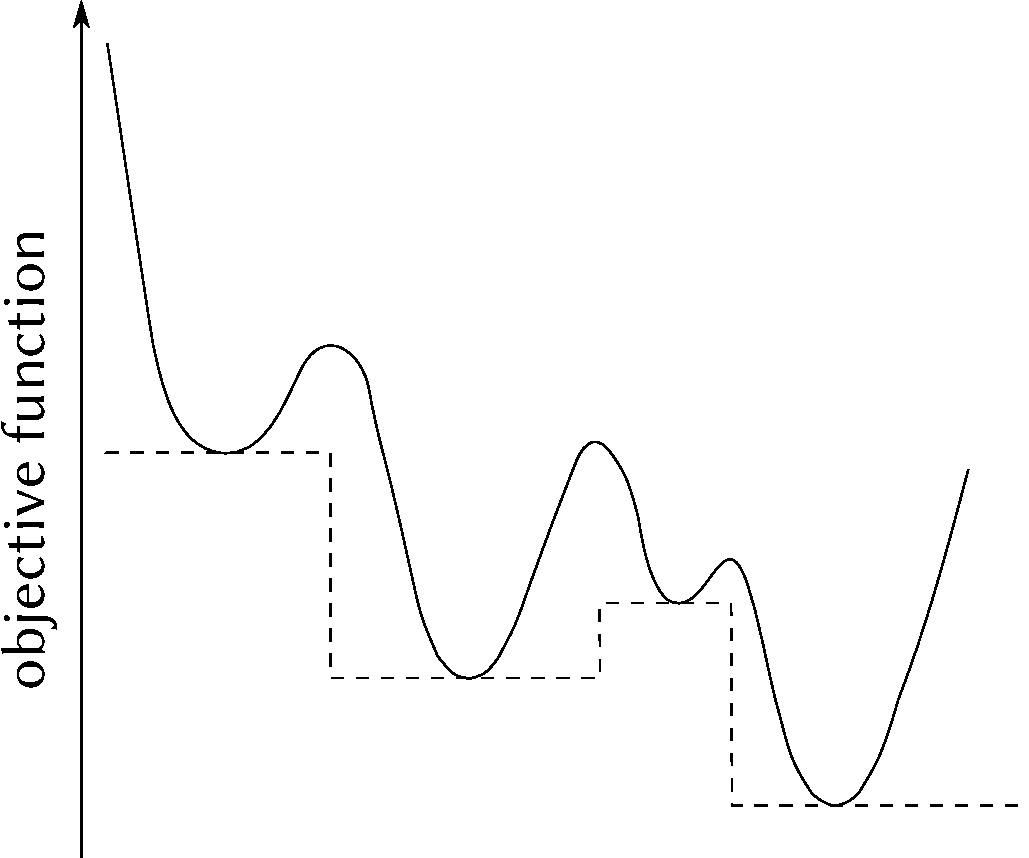
\includegraphics[width=.8\textwidth]{other-pics/basin-hopping.pdf}
    \caption{Hypersurface transformation in the basin-hopping method. The original hypersurface (solid line) is mapped onto the transformed surface (dashed line) by a geometry optimisation.}
    \label{fig:PEStransform}
\end{figure}
%
The mapping procedure is usually combined with a Monte-Carlo-type sampling
procedure.\autocite{Wales_GlobalOptimizationBasinHopping_1997} A new sample is
created by introducing a small random displacement, analogous to the simulated
annealing approach, followed by a geometry optimisation. The acceptance of the
result is, again, determined by the Metropolis criterion. The effect of the
transformation is that transition states are removed from the hypersurface and
dynamics are accelerated as local minima can be left easily by fixing the
acceptance ratio to the desired value via the effective temperature in the
Metropolis step. Contrary to the simulated annealing method, the basin-hopping
approach is capable of finding the global minimum even on hypersurfaces with
multiple almost degenerate low-lying minima.
%
\\\newline
In the \textit{genetic algorithm}
approach\autocite{Goldberg_GeneticAlgorithmsSearch_1989} the hypersurface is
explored by utilizing ideas from evolution theory, in particular natural
selection. A ``gene'' is represented by the coordinates of the particles,
forming a ``chromosome''. The ``fitness'' of a structure is determined by the
potential energy with respect to the objective function. The structural
information is often encoded in a binary bit string, but it is also possible to
just use coordinates directly. In the first step of the algorithm an initial
population is generated randomly and their fitness is calculated. A pair of
``parents'' is chosen, on of which is picked randomly while the other is
selected based on its fitness. The structures of the parents are combined to
create two ``children'' with a fixed probability of a single bit to cross-over.
Additionally, a low probability for random mutations is incorporated into the
algorithm as well. After the next generation is created the parent generation is
discarded to leave the population size constant. The algorithm is inherently
parallel as multiple pairs of parents can be treated simultaneously. In its
first application to clusters it was shown that a genetic algorithm can lead to
convergence towards the global minimum in far fewer steps than for example the
simulated annealing method.\autocite{Hartke_Globalgeometryoptimization_1993}

The algorithms mentioned in this section represent only a subset of all
available global optimisation methods for the search of stationary points on a
\ac{PES}. Other algorithms that can be used to solve the problem at hand are,
for example, the particle swarm algorithm or the ant colony optimisation method.

\acresetall

\chapter{Interaction Potentials}
\label{sec:energylandscapes}

Systems of large numbers of atoms or complete scans of potential hypersurfaces
are usually not treatable by accurate quantum chemical methods as introduced in
chapter~\ref{sec:basicsofQC}. In those cases more simple interaction potentials have to be
employed, without loosing crucial information about the system. In the following
sections two potentials used in this thesis will be introduced. If not noted
otherwise the following sections are based on a book by
\citeauthor{Hirschfelder_Moleculartheorygases_1964}.\autocite{Hirschfelder_Moleculartheorygases_1964} 

\section{Thermodynamic Considerations}
\label{sec:ThermodynamicConsiderations}

The need to find intermolecular interaction potentials arose from the desire to
have a good description for the equation of state of a gas. A purely empirical
relation was first found by
\citeauthor{KamerlinghOnnes_Expressionequationstate_1902}.\autocite{KamerlinghOnnes_Expressionequationstate_1902}
%
\begin{align}
    pv=A'+\frac{B'}{v}+\frac{C'}{v^2}+\frac{D'}{v^4}+\frac{E'}{v^6}+\frac{F'}{v^8}
\end{align}
%
Here, $p$ represents the pressure of the gas, $v$ the molar volume of the
container and the parameters $A'$ to $F'$ are the \textit{virial coefficients}.
The latter are functions of temperature $T$ and can be adjusted to fit the
polynomial to experimental data obtained from various gases. It is often
sufficient to focus on the first three virial coefficients to obtain a useful
equation of state. 

This formulation can be generalised in terms of Taylor expansion
%
\begin{align}
    \frac{pv}{RT}=1+\frac{B}{v}+\frac{C}{v^2}+\frac{D}{v^3}+\dots,\label{eqn:VirialEquationOfState}
\end{align}
%
which allows the virial coefficients\footnote{Note that the prime notation was
dropped to emphasise that the virial coefficients in this equation are different
to the ones originally proposed in equation~\eqref{eqn:VirialEquationOfState}.}
to be expressed as functions of intermolecular potentials. If all virial
coefficients are 0, equation~\eqref{eqn:VirialEquationOfState} is equal to the
ideal gas equation, which means that the virial coefficients are connected to
the interactions between gas molecules not included in the ideal gas law.
Analytic expressions for the virial coefficients can be derived as explained in
the following section. It is clear that this expansion converges if the virial
coefficients are small compared to the volume $v$.

\subsection{Equation of State from the Partition Function}
\label{sec:equationofstatefromthepartitionfunction}

The partition function $Z_N$ can be used to derive various thermodynamic
quantities, for instance the pressure $p$.
%
\begin{align}
    p=kT\left(\pdv{\ln Z_N}{V}\right)_T\label{eqn:PressureEquationOfState}
\end{align}
%
In this equation, $k$ is the Boltzmann constant, $T$ the temperature and $V$ the
volume of the vessel. Using the expression of the classical partition function
for a system of $N$ identical particles\footnote{See page 106 in reference
\cite{Hirschfelder_Moleculartheorygases_1964}.} the partition function can be
re-formulated in terms of Boltzmann factors
$W_N\left(\mathbf{r}^N\right)=e^{-\beta\Phi\left(\mathbf{r}^N\right)}$ and a
configurational integral $Q_N$.
%
\begin{align}
    Q_N&=\frac{1}{N!}\int W_N\left(\mathbf{r}^N\right)\dd{\mathbf{r}^N}\label{eqn:ConfigurationalIntegral}\\
    Z_N&=\frac{Q_N}{\lambda^{3N}}\,\text{with}\, \lambda^2=\frac{h^2}{2\pi mkT}\label{eqn:PartitionFunction}
\end{align}
%
Here, $\mathbf{r}^N$ refers to the set of coordinates defined by the set of $N$
molecules, $h$ is Planck's constant, $m$ the particle mass and $\beta=1/kT$. The
potential function $\Phi\left(\mathbf{r}^N\right)$ depends on all particle
coordinates and is not yet defined explicitly. However, expressions for the
virial coefficients can be found without defining the interaction potential by
using a method introduced by
\citeauthor{Ursell_evaluationGibbsphaseintegral_1927}\autocite{Ursell_evaluationGibbsphaseintegral_1927}.
This method requires the definition of ``U-functions''
$U_l\left(\mathbf{r}^\lambda\right)$ that are expressed as combinations of
Boltzmann factors. The subscript $l$ refers to how many molecules the U-function
includes and $\lambda$ denotes which molecules. For example, the first two
U-functions are defined as:
%
\begin{align}
    U_1\left(\mathbf{r}_i\right)&=W_1\left(\mathbf{r}_i\right)\\
    U_2\left(\mathbf{r}_i,\mathbf{r}_j\right)&=W_2\left(\mathbf{r}_i,\mathbf{r}_j\right)-W_1\left(\mathbf{r}_i\right)W_1\left(\mathbf{r}_j\right).
\end{align}
%
The advantage of using these expression can be demonstrated by considering the
condition under which $U_l\left(\mathbf{r}^\lambda\right)$ vanishes. For
example, for the second U-function to be equal to zero, both terms containing
Boltzmann factors must be equal.
%
\begin{align}
    W_2\left(\mathbf{r}_i,\mathbf{r}_j\right)&=W_1\left(\mathbf{r}_i\right)W_1\left(\mathbf{r}_j\right)\\
    \Phi\left(\mathbf{r}_i,\mathbf{r}_j\right)&=\Phi\left(\mathbf{r}_i\right)+\Phi\left(\mathbf{r}_j\right)
\end{align}
%
The latter is true if the molecules $i$ and $j$ are sufficiently far apart for
their interaction to be negligible. For the higher order U-functions this
concept can be extended to two or more groups of molecules being far enough
apart for their interaction to become 0. By reversing the definition of the
U-functions, the Boltzmann factors can be expressed in terms of U-functions.
%
\begin{align}
    W_N\left(\mathbf{r}^N\right)=\sum_{\sum lm_l=N}\prod U_l\left(\mathbf{r}^\lambda\right)
\end{align}
%
The summation has to be carried out over all divisions of $N$ molecules into
$m_l$ groups of $l$ molecules. With this expression
equation~\eqref{eqn:ConfigurationalIntegral} can now be solved.
%
\begin{align}
    Q_N = \sum_{\sum lm_l=N} \prod_{l=1}^N\frac{(Vb_l)^{m_l}}{m_l!}\label{eqn:ConfigurationIntegralbl}
\end{align}
%
The U-functions are now included in the \textit{cluster integrals} $b_l$ which
are defined in the following way.
%
\begin{align}
    b_l=\left(Vl!\right)^{-1}\int U_l(\mathbf{r}_1,\mathbf{r}_2,\dots,\mathbf{r}_l)\dd{\mathbf{r}_1}\dd{\mathbf{r}_2}\dots\dd{\mathbf{r}_l}
\end{align}
%
Equation~\eqref{eqn:PartitionFunction} can now be expressed in terms of the
cluster integrals and the equation of state in virial form can be derived from
equation~\eqref{eqn:PressureEquationOfState}.
%
\begin{align}
    \ln Z_N=-N\ln z\lambda^3 + \sum_{l=1}^\infty Vb_lz^l\\
    pV=kTV\left(\pdv{\ln Z_N}{V}\right)_T=kT\sum_lVb_lz^l\\
    z=\frac{N}{V}\exp\left(-\sum_{i=1}^\infty\gamma_i\left(\frac{N}{V}\right)^i\right)
\end{align}
%
Here, $z$ has the dimension of a concentration and is called the \textit{active
number density}. $\gamma_i$ are combinations of cluster integrals and the first
two are
%
\begin{align}
    \gamma_1&=2b_2\\
    \gamma_2&=3b_3-6b_2^2.
\end{align}
%
Combining the equations above leads to an equation similar to
equation~\eqref{eqn:VirialEquationOfState}.
%
\begin{align}
    \frac{pv}{RT}=1-\sum_{i=1}^\infty\frac{i\gamma_i}{i+1}\left(\frac{N}{V}\right)^i\label{eqn:VirialEquationOfStateClusterIntegrals}
\end{align}
%
Comparing equations~\eqref{eqn:VirialEquationOfState} and
\eqref{eqn:VirialEquationOfStateClusterIntegrals} it is clear that the virial
coefficients can be expressed in terms of cluster integrals.
%
\begin{align}
    B(T)&=-\frac{1}{2}N_A\gamma_1\\
    C(T)&=-\frac{2}{3}N_A^2\gamma_2
\end{align}
%
As stated before, the virial coefficients arise from the molecular interactions
as they are functions of the cluster integrals that in turn consist of
many-body interactions. Additionally, it can be seen, that the second virial
coefficient $B$ depends only on two-body interactions, the third virial
coefficient $C$ on two- and three-body interactions and so on.

Further simplification can be achieved by the assumption of additivity, which
allows the total potential energy of the system to be expressed in terms of
pairwise interactions $\varphi_{ij}$.
%
\begin{align}
    \Phi\left(\mathbf{r}^N\right)=\frac{1}{2}\sum_i\sum_j\varphi_{ij}
\end{align}
%
The magnitude of the error introduced by this treatment has been calculated by
\citeauthor{Axilrod_InteractionvanWaals_1943}\autocite{Axilrod_InteractionvanWaals_1943}
to scale with $r^{-9}$. The U-functions can now be expressed in terms of
modified Boltzmann factors $f_{ij}(r_{ij})$, which are defined such that they only differ from
zero if the interaction energy is significant.
%
\begin{align}
    f_{ij}(r_{ij})=e^{-\beta\varphi_{ij}}-1
\end{align}
%
For the U-functions this results in the following expressions.
%
\begin{align}
    \begin{aligned}
    U_1(\mathbf{r}_1)&=1\\
    U_2(\mathbf{r}_1,\mathbf{r}_2)&=f_{12}\\
    U_3(\mathbf{r}_1,\mathbf{r}_2,\mathbf{r}_3)&=f_{12}f_{23}f_{13}+f_{12}f_{23}+f_{23}f_{13}+f_{12}f_{23}
    \end{aligned}
\end{align}
%
From these definitions, expressions depending on two-body interactions for the
virial coefficients can be derived.
%
\begin{align}
    B(T)=-\frac{2\pi N}{3kT}\int\limits_0^\infty r^3\dv{\varphi}{r}e^{-\beta\varphi(r)}\dd{r}
\end{align}
%
In diluted gases, where interactions of more than two particles are rare, an
equation of state only containing the second virial coefficient describes
the system well enough.
%
\begin{align}
    \frac{pv}{RT}=1+\frac{B}{v}
\end{align}
%

\section{Lennard-Jones Potential}
\label{sec:LennardJones}

One of the most widely used interaction potentials today is the \acf{LJ}
potential. It was first introduced by
\citeauthor{Jones_DeterminationMolecularFields_1924} (later Lennard-Jones) on
April 22, 1924\autocite{Jones_DeterminationMolecularFields_1924}, however, the
same potential was submitted for publication by
\citeauthor{Simon_KristallstrukturArgons_1924} only a few days
later.\autocite{Simon_KristallstrukturArgons_1924} The potential introduced by
Lennard-Jones depending on the distance $r$ between two objects was of the form
%
\begin{align}
    V_{m,n}^\text{LJ}(r)=\frac{\lambda_n}{r^n}-\frac{\lambda_m}{r^m},\, m<n,\label{eqn:LJgeneral}
\end{align}
%
with $m$ and $n$ not being set at that time. However, even though this general
potential form is nowadays known as the Lennard-Jones potential, there had been
other attempts at defining similar interaction potentials earlier. In 1920,
\citeauthor{Kratzer_ultrarotenRotationsspektrenHalogenwasserstoffe_1920}\autocite{Kratzer_ultrarotenRotationsspektrenHalogenwasserstoffe_1920}
already published a less general potential of the same form with the exponents
$m$ and $n$ set to 1 and 2, respectively. The general idea behind these two
potential forms was already discussed earlier in the beginning of the 20th
century by
\citeauthor{Mie_ZurkinetischenTheorie_1903}\autocite{Mie_ZurkinetischenTheorie_1903}.
In all those potentials attractive and repulsive distance dependent terms are
combined such that the resulting potential energy function has a minimum value
at some equilibrium distance. For distances larger than the equilibrium distance
the potentials approach zero asymptotically from below, while they diverge
towards $+\infty$ for distances close to zero.

Lennard-Jones used this potential form to solve the integral expression in the
second virial coefficient $B$. Analytical expressions can also be found for
purely repulsive potentials and the attractive Sutherland potential.
Lennard-Jones, however, introduced the potential in
equation~\eqref{eqn:LJgeneral} and solved the equation of state analytically to
derive parameters for $\lambda_n$ and $\lambda_m$ based on experimental results
for noble gases\autocite{Jones_DeterminationMolecularFields_1924} and later on
for the solid state.\autocite{Jones_calculationcertaincrystal_1925}

Equation~\eqref{eqn:LJgeneral} can be redefined in terms of parameters for the
depth of the potential energy well $\varepsilon$ and equilibrium distance
$r_e$. Under the constraint of $V_{m,n}(r_e)=-\varepsilon$ and
$\dv{V_{m,n}(r_e)}{r}=0$ a more common notation of the \ac{LJ} potential can be
derived.
%
\begin{align}
    V_{m,n}^\text{LJ}(r)=\frac{\varepsilon}{n-m} \left[ m \left(\frac{r_e}{r}\right)^n  - n\left(\frac{r_e}{r}\right)^m \right]\label{eqn:LJgeneral_theory}
\end{align}
%
Both parameters $\varepsilon$ and $r_e$ can be determined by the size of the
interacting atoms and the interaction strength. The evaluation of the exponents
$m$ and $n$, however, is more complicated. The exponent $m$ is mainly important
for the correct long range behaviour, while $n$ dominates for distances smaller
than $r_e$. First attempts at deriving the correct long range behaviour have
been made by considering two hydrogen
atoms.\autocite{Wang_gegenseitigeEinwirkungzweier_1927} The attractive force was
shown to scale with $r^{-7}$, which is in agreement with other investigations,
showing the \textit{potential} of the attractive field\footnote{Note that the
force is the first derivative of the potential.} to be on the order of
$r^{-6}$.\autocite{Eisenschitz_UeberVerhaeltnisvan_1930,Lennard-Jones_Perturbationproblemsquantum_1930,Hasse_calculationvanWaal_1931,Slater_VanWaalsForces_1931}
First attempts were made to relate the long-range behaviour to the
polarisability of the
atoms,\autocite{London_ZurTheorieund_1930,Slater_VanWaalsForces_1931} a
correlation that is used to treat van-der-Waals interactions parametrically,
today (see section~\ref{sec:dispersioncorrections}). Lennard-Jones calculated
force constants for various gases showing the same long-range behaviour from
studying their equation of
state.\autocite{Jones_DeterminationMolecularFields_1924,Jones_atomicfieldshelium_1925,Lennard-Jones_theoreticalcalculationsphysical_1925,Lennard-Jones_molecularfieldshydrogen_1926,Lennard-Jones_equationstategaseous_1927}

The repulsive part is more complicated, as it can not be derived directly from
the equation of state. Lennard-Jones used lattice parameters and heats of
sublimation from experiments to fit his potential. He found $n=12$ and $m=6$ to
fit the data well, giving rise to the most commonly used form of the \ac{LJ}
potential: $V_{6,12}(r)$.\autocite{Lennard-Jones_Cohesion_1931} Some examples
for potential curves with exponents $n=12$ and $m=6$ can be found in
figure~\ref{fig:LJ-param}.
%
\begin{figure}[htb]
    \centering
    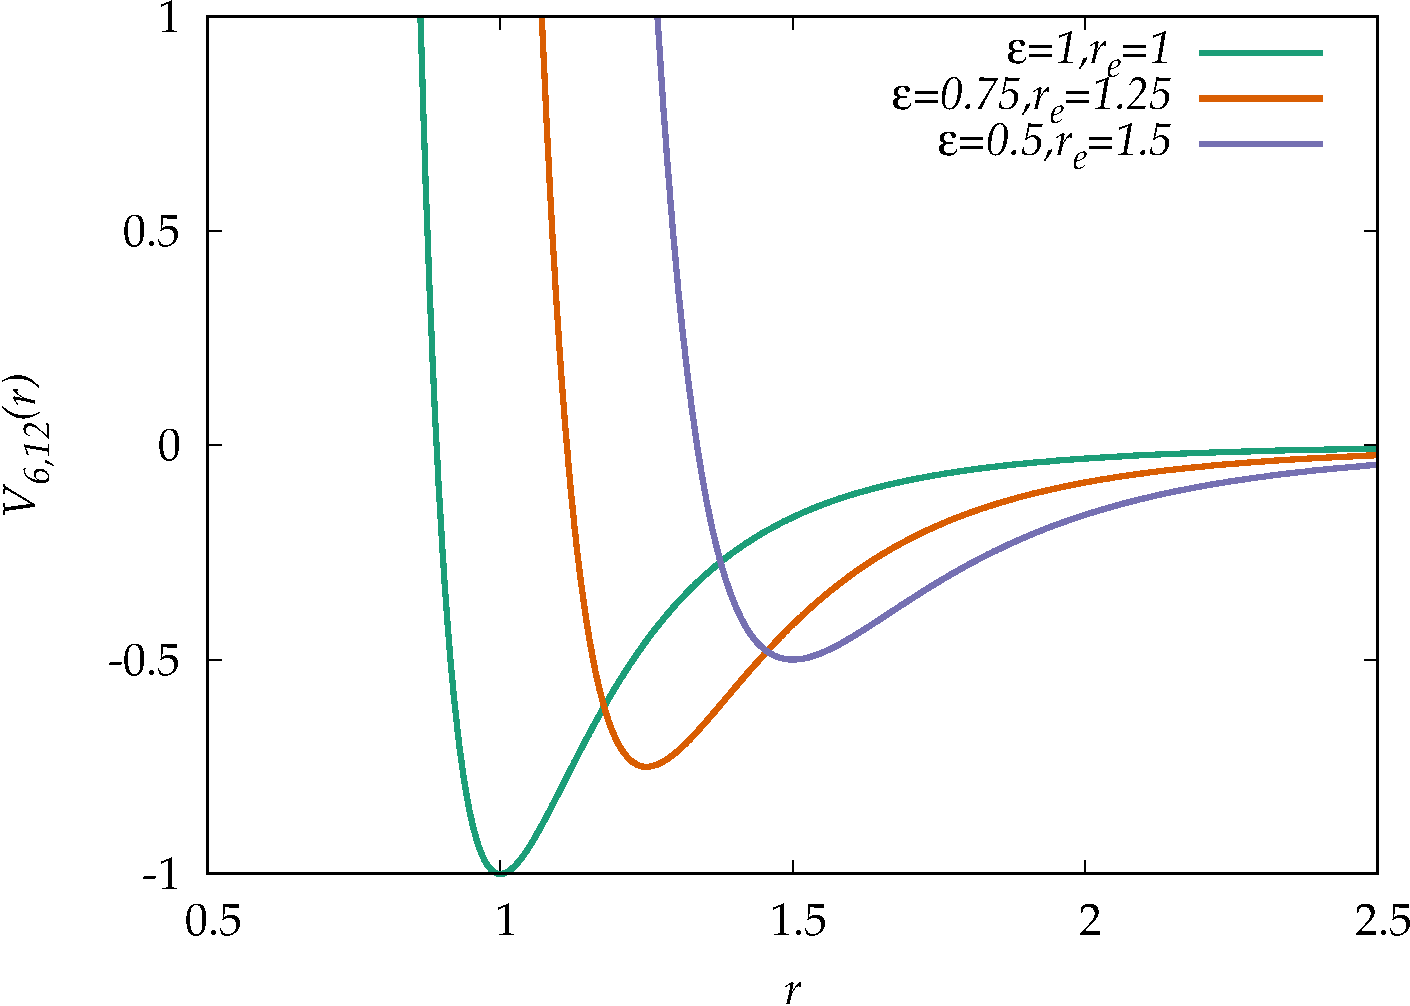
\includegraphics[width=.8\textwidth]{plot/LJ-param.pdf}
    \caption{Examples of Lennard-Jones potential curves for the (6,12)-\acs{LJ}
    potential with different values for $\varepsilon$ and $r_e$.}
    \label{fig:LJ-param}
\end{figure}

\subsection{Extended Lennard-Jones Potential}
\label{sec:eLJ}

A more sophisticated solution to describing intermolecular interactions can
be achieved with the \acf{eLJ} potential. The choice of the exponents $m$ and $n$ in
the \ac{LJ} potential is arbitrary and lacks flexibility. Any effect that scales
differently from $r^{-12}$ or $r^{-6}$ can not be described accurately.
Therefore, it seems almost natural to extend the \ac{LJ} potential by a sum over
different $r^{-i}$ terms weighted by coefficients $c_i$.
%
\begin{align}
    V_\text{eLJ}(r)=\sum_{i=n_\text{min}}^{n_\text{max}} c_{i}r^{-i}\label{eqn:ELJ}
\end{align}
%
The number and type of the exponents $n_\text{min}$ to $n_\text{max}$ needs to
be determined based on the investigated system. For example, in the original
publication only even exponents from 6 to 16 were
included.\autocite{Schwerdtfeger_ExtensionLennardJonespotential_2006} A later
study investigated the Xenon dimer and it was decided to include exponents up to
$i=18$ and also some odd numbered
ones.\autocite{Jerabek_relativisticcoupledclusterinteraction_2017} In both cases
the coefficients $c_i$ are determined by a fitting procedure to very accurate
dissociation curves of the respective dimer molecules calculated by
coupled-cluster theory. For such a potential the cohesive energy of the solid
state can be expressed analytically in terms of lattice
sums.\autocite{Schwerdtfeger_ExtensionLennardJonespotential_2006}

\subsection{Lennard-Jones Clusters}
\label{sec:LJClusters}

The \ac{LJ} potential has been used extensively to study nucleation of clusters
and as a benchmark for global optimisation methods
(section~\ref{sec:GlobalOptimisation}). From the derivation of the \ac{LJ}
potential as a interaction potential to obtain analytical solutions for the second
virial coefficient, it should be clear that it is a rather crude approximation
for the forces between atoms in a cluster of the size of a few atoms.
Nevertheless, the \ac{LJ} potential is capable of making verifiable predictions
especially in the case of the rare gas
clusters.\autocite{Wales_Energylandscapes_2003} For example, the most stable
arrangement is often predicted to be a Mackay icosahedron in agreement with
experimental results.\autocite{Kakar_SizedependentKedgeEXAFS_1997} The reason
for this agreement lies within the nature of the interaction between rare gas
atoms due to dispersive forces, which are approximated well by the \ac{LJ}
potential.

The hypersurface upon which the particles move, also called a \acf{PES} or energy
landscape, has been explored extensively for the \ac{LJ} potential.
\autocite{Tsai_Useeigenmodemethod_1993,Ball_Dynamicsstatisticalsamples_1999,Doye_Saddlepointsdynamics_2002} \citeauthor{Doye_Saddlepointsdynamics_2002}\autocite{Doye_Saddlepointsdynamics_2002}
employed the eigenvector following method (section~\ref{sec:GOAlgorithms}) to
find an initial set of minima and transition states with Hessian index
1.\footnote{The Hessian index gives the number of negative eigenvalues of the
Hessian matrix.} From this set higher order Hessian index saddle point can be
found by randomly perturbing the found minima and transition states and
following the eigenvector to a new stationary point. Additionally, stationary
points were searched for in reverse order, meaning the search was started from a
high order index saddle point and structures with lower Hessian index were
located by perturbing the initial structure randomly.

Absolute numbers of local minima of \ac{LJ} clusters can be found in the results
part (table~\ref{tab:comp}, page~\pageref{tab:comp}).

\section{Sticky-Hard-Sphere Potential}
\label{sec:SHS}

%The \acf{SHS} potential was originally introduced by
%\citeauthor{baxter68}\autocite{baxter68} to derive an analytical solution to
%Ornstein-Zernike relation\autocite{Ornstein_Accidentaldeviationsdensity_1914}
%with a correlation function as proposed by
%\citeauthor{Percus_AnalysisClassicalStatistical_1958}\autocite%{Percus_AnalysisClassicalStatistical_1958}
%The Ornstein-Zernike relation allows to measure the influence of one particle to
%another one in terms of their distance. The indirect correlation function $h%(\mathbf{r})$
%is often defined in terms of the radial distribution function $g(\mathbf{r})$.
%%
%\begin{align}
%    h(\mathbf{r})=g(\mathbf{r})-1
%\end{align}
%%
%In the Ornstein-Zernike approximation $h(\mathbf{r})$ as 
%%
%\begin{align}
%    h(\mathbf{r})=c(\mathbf{r})+\rho\int\dd{\mathbf{r'}}c(|\mathbf{r'}|)h(|\mathbf%{r}-\mathbf{r'}|).
%\end{align}
%%
%Here, $\rho$ is the particle density and $h(\mathbf{r})$ describes the
%probability of finding a second particle at the distance $r$ to a particle at
%the origin. As derived by \citeauthor{Percus_AnalysisClassicalStatistical_1958}
%the direct correlation function is
%$c(\mathbf{r})=g(\mathbf{r})\left(1-\exp{\phi(\mathbf{r})/kT}\right)$. For the %potential term $\phi(r)$ Baxter introduced a potential for hard spheres with %surface adhesion, which can be expressed as
%
A variation of the \acf{SHS} potential was originally introduced by
\citeauthor{baxter68}\autocite{baxter68} and can be regarded as a rigid sphere
interaction with surface adhesion. In the simpler rigid sphere model the
interaction potential is 0 for distances larger than the equilibrium distance
$r_s$ and goes to infinity when the particles ``touch''. The rigid sphere model
with surface adhesion builds upon this by introducing a region of
attraction of width $R(r_s-1)$ in which the potential is defined to be $-\varepsilon$.
The potential can be defined as
%
\begin{align}
    V^\text{SW}(r) =
    \begin{cases}
        \infty & 0 < r < r_s.\\
        -\varepsilon & r_s < r < Rr_s.\\
        0 & r > Rr_s.
    \end{cases}
\end{align}
%
For this potential the second and third virial coefficients have been evaluated
analytically. For clarity only the more important second virial coefficient
$B(T)$ is shown.
%
\begin{align}
    B(T)=\frac{2}{3}\pi N_A{r_s}^3\left[1-(R^3-1)\left(\exp{\frac{\varepsilon}{kT}}-1\right)\right]
\end{align}
%
Interestingly, this potential shows a relationship to the (6,12)-\ac{LJ}
potential. For values of $R=1.8$ and $\varepsilon = 0.56$ the second virial
coefficient becomes
%
\begin{align}
    B(T)=\frac{2}{3}\pi N_A{r_s}^3\left(1-4.832\left(\exp{\frac{\varepsilon}{kT}}-1\right)\right),
\end{align}
%
which approximates the second virial coefficient of the (6,12)-\ac{LJ} potential
quite well.\autocite{Hirschfelder_Moleculartheorygases_1964}

More important for the scope of this thesis is, however, the relation to the
\ac{LJ} potential for when the width of the potential well goes to 0. In this
case the potential can be written as
%
\begin{align}
    V^\text{SHS}(r) =
    \begin{cases}
        \infty & 0 < r < r_s,\\
        -\varepsilon & r=r_s,\\
        0 & r > r_s,
    \end{cases}\label{eqn:SHSpotential}
\end{align}
%
which is then often called the \ac{SHS} potential. If the \ac{LJ} potential is
expressed in terms of equation~\eqref{eqn:LJgeneral_theory},
equation~\eqref{eqn:SHSpotential} represents the limit with respect to the
exponents $(n,m)$ approaching infinity.\footnote{An illustration of this
property is shown in figure~\ref{fig:LJ}.}
%
\begin{align}
    \lim_{m,n\to\infty} V_{m,n}^\text{LJ} = V^\text{SHS}
\end{align}
%
This can easily be shown by applying l'H\^opital's rule to
equation~\eqref{eqn:LJgeneral_theory} and deriving the limits for the cases
presented in equation~\eqref{eqn:SHSpotential}.

\subsection{Sticky Hard Sphere Clusters}
\label{sec:SHSClusters}

Similar to the \ac{LJ} clusters, the \ac{SHS} clusters can be found by
investigating combinations of spheres that minimise the potential in
equation~\eqref{eqn:SHSpotential}. As the \ac{SHS} potential is not a continuous
function, common optimisation algorithms can not be used to investigate the potential
energy landscape. However, the nature of the \ac{SHS} potential results in a
neat property that allows the clusters to be defined in terms of graph theory.
Only pairs of spheres that have the right distance of $r=r_s$ contribute to the
overall energy, allowing the energy to be expressed in terms of the contact
number $N_c$.
%
\begin{align}
    E=-\varepsilon N_c=-\varepsilon \sum\limits_{i>j} A_{ij}
\end{align}
%
This allows the clusters to be represented by adjacency matrices $\mathbf{A}$,
where a contact state is represented by a matrix element of $A_{ij}=1$
and every other position by
$A_{ij}=0$.\autocite{Arkus_DerivingFiniteSphere_2011} The problem of
minimising the energy now becomes a problem of maximising the contact number
$N_c$, or the number of 1 entries in the adjacency matrix. The adjacency matrix
of a cluster will be symmetric, which means there are $2^{N(N- 1)/2}$ different
combinations that could all potentially represent a cluster structure. To find
all possible packings, all adjacency matrices have to be analysed with respect
to their suitability for a stable cluster structure, a method called
\textit{exact enumeration}. A large number of possible adjacency matrices can be
rejected immediately, because they represent an already found structure with a
different particle labelling. This particle labelling degeneracy is due to the
fact that the spheres are all equal and therefore swapping two rows or columns
in the adjacency matrix will not change the underlying cluster structure. If two
adjacency matrices correspond to the same structure they are said to be
\textit{isomorphic} (see chapter~\ref{sec:DefinitionGraph}).

Besides the obvious rejection of adjacency matrices that are isomorphic, other
restrictions can be imposed to reduce the numbers of adjacency matrices further.
Most importantly, the resulting structures should be rigid, meaning not
continuously deformable. Thus, each sphere needs to be in contact with at least
three other spheres, which is true if each row or column of the adjacency matrix
contains at least three matrix elements of 1. Another restriction that has often
been imposed on the adjacency matrices is the Maxwell criterion, which states
that the contact number needs to fulfil $N_c\geq 3N-6$ for a structure to be
rigid.\autocite{Maxwell_calculationequilibriumstiffness_1864} However, recent
investigations revealed the existence of rigid structures with $N_c<
3N-6$.\autocite{Holmes-Cerfon_EnumeratingRigidSphere_2016} Up to a size of $N=4$
all inter-particle distances are completely defined by the adjacency matrix.
Starting from $N=5$ there will be at least one unknown inter-particle distance,
which needs to be determined algebraically. For this, the distance matrix
$\mathbf{D}$ needs to be constructed from the adjacency matrix. This can be
achieved by defining $3N-6$ equations (and $N(N-1)/2 - (3N-6)$ inequalities)
from the adjacency information.
%
\begin{align}
    A_{ij}=1\rightarrow r_{ij}=2r\\
    A_{ij}=0\rightarrow r_{ij}>2r
\end{align}
%
The system has $3N$ variable coordinates, but by fixing one sphere at the origin
of the coordinate system and a second one along one of the coordinate axis, the
number can be reduced to $3N-6$, and the system is completely defined by the
equations above. In case the structure has more contacts than $3N-6$ the system
is overdefined, but still solvable. Deriving an efficient method for mapping the
adjacency matrix into the distance matrix is the crucial step to examine
clusters bound by the \ac{SHS} potential.

A set of geometric elimination rules and distance rules have been derived by
\citeauthor{Arkus_DerivingFiniteSphere_2011}\autocite{Arkus_DerivingFiniteSphere_2011}.
An elimination rule sorts out unphysical adjacency matrices, while a distance
rule solves for the mapping $A_{ij}\to D_{ij}$. These rules
can be derived from geometric considerations about the neighbourhood of a
sphere. If another sphere touches a sphere of radius $r$, it must lie on the
surface of a sphere with radius $R=2r$. For two spheres in contact, their
surrounding spheres intersect and form an \textit{intersection circle} with
radius $\frac{\sqrt{3}}{2}R$. Therefore, each matrix element $A_{ij}$
can be related to and intersection circle between spheres $i$ and $j$. Several
rules can be derived from considering the intersection circles of the particles,
for instance, the fact that more than one intersection circle can only intersect
in 0, 1 or 2 points (and never more) implies that three connected spheres can
never be touched by more than two spheres simultaneously. The article by
\citeauthor{Arkus_DerivingFiniteSphere_2011} referenced above contains many more
such rules that can be used to construct \ac{SHS} clusters.

Results for complete exact enumeration of up to 14
spheres\autocite{Arkus_DerivingFiniteSphere_2011,Hoy_Structurefinitesphere_2012,Hoy_Structuredynamicsmodel_2015,Holmes-Cerfon_EnumeratingRigidSphere_2016}
have been published. The results by
\citeauthor{Holmes-Cerfon_EnumeratingRigidSphere_2016}\autocite{Holmes-Cerfon_EnumeratingRigidSphere_2016}
also showed evidence of so called hypostatic clusters with less than $3N-6$
contacts. This is due to the fact that in this study a modification of the exact
enumeration method was used, which follows one-dimensional transition paths
created from breaking a random contact in an already found cluster. Another
interesting find in this publication was the existence of clusters that share
the same adjacency matrix representation. This means that the mapping from
adjacency matrix to cluster embedding is not a bijection, but only surjective.
An overview of these results can be found in table~\ref{tab:comp}
(page~\pageref{tab:comp}).